\chapter{Mathematical Background}\label{chapmath}

\begin{objectives} \label[objectives]{Recall-basic-mathematical}

\begin{itemize}
\tightlist
\item
  Recall basic mathematical notions such as sets, functions, numbers,
  logical operators and quantifiers, strings, and graphs.
\item
  Rigorously define Big-\(O\) notation.
\item
  Proofs by induction.
\item
  Practice with reading mathematical \emph{definitions},
  \emph{statements}, and \emph{proofs}.
\item
  Transform an intuitive argument into a rigorous proof.
\end{itemize}

\end{objectives}

\begin{quote}
\emph{``I found that every number, which may be expressed from one to
ten, surpasses the preceding by one unit: afterwards the ten is doubled
or tripled \ldots{} until a hundred; then the hundred is doubled and
tripled in the same manner as the units and the tens \ldots{} and so
forth to the utmost limit of numeration.''}, Muhammad ibn Mūsā
al-Khwārizmī, 820, translation by Fredric Rosen, 1831.
\end{quote}

In this chapter we review some of the mathematical concepts that we use
in this book. These concepts are typically covered in courses or
textbooks on ``mathematics for computer science'' or ``discrete
mathematics''; see the ``Bibliographical Notes'' section
(\cref{notesmathchap}) for several excellent resources on these topics
that are freely-available online.

\emph{A mathematician's apology.} Some students might wonder why this
book contains so much math. Mathematics is a language for modeling
concepts in a precise and unambiguous way. In this book we use math to
model the concept of \emph{computation}. For example, we will consider
questions such as \emph{``is there an efficient algorithm to find the
prime factors of a given integer?''}. (We will see that this question is
particularly interesting, touching on areas as far apart as Internet
security and quantum mechanics!) To even \emph{phrase} such a question,
we need to give a precise \emph{definition} of the notion of an
\emph{algorithm}, and of what it means for an algorithm to be
\emph{efficient}. Also, since there is no empirical experiment that will
prove the \emph{nonexistence} of an algorithm, the only way to establish
such a result is using a \emph{mathematical proof}.

\section{This chapter: a reader's manual}\label{manualbackground}

Depending on your background, you can approach this chapter in two
different ways:

\begin{itemize}
\item
  If you already have taken a ``discrete mathematics'', ``mathematics
  for computer science'' or similar courses, you can take a quick look
  at \cref{secmathoverview} to see the main tools we will use,
  \cref{notationsec} for our notation and conventions, and then skip
  ahead to the rest of this book. Alternatively, you can sit back,
  relax, and read this chapter just to get familiar with our notation,
  as well as to enjoy (or not) my philosophical musings and attempts at
  humor. You might also want to start brushing up on \emph{discrete
  probability}, which we'll use later in this book.
\item
  If your background is less extensive, see \cref{notesmathchap} for
  some resources on these topics. This chapter briefly covers the
  concepts that we need, but you may find it helpful to see a more
  in-depth treatment. As usual with math, the best way to get comfort
  with this material is to work out exercises on your own.
\end{itemize}

\section{A quick overview of mathematical
prerequisites}\label{secmathoverview}

The main mathematical concepts we use in this book are:

\begin{itemize}
\item
  \textbf{Proofs:} First and foremost, this book involves a heavy dose
  of formal mathematical reasoning, which includes mathematical
  \emph{definitions}, \emph{statements}, and \emph{proofs}.
\item
  \textbf{Sets:} The basic set \emph{relations} of membership (\(\in\))
  and containment (\(\subseteq\)), and set \emph{operations},
  principally union (\(\cup\)), intersection (\(\cap\)), set difference
  (\(\setminus\)) and Cartesian product (\(\times\)).
\item
  \textbf{Tuples and strings:} The set \(\Sigma^k\) of length-\(k\)
  strings/lists over elements in \(\Sigma\), where \(\Sigma\) is some
  finite set which is called the \emph{alphabet} (quite often
  \(\Sigma = \{0,1\}\)). We use \(\Sigma^*\) for the set of all strings
  of finite length.
\item
  \textbf{Some special sets:} The set \(\N\) of natural numbers.
  Following typical computer science convention, our indices start from
  zero and so we write \(\N = \{0,1,2,\ldots \}\). We use \([n]\) for
  the set \(\{0,1,2,\ldots,n-1\}\). We use \(\{0,1\}^*\) for the set of
  all binary strings and \(\{0,1\}^n\) for the set of strings of length
  \(n\) for some natural number \(n\in\N\). If \(x\) is a string of
  length \(n\), then we refer to its elements by \(x_0,\ldots,x_{n-1}\).
\item
  \textbf{Functions:} The \emph{domain} and \emph{codomain} of a
  function, properties such as being \emph{one-to-one} (also known as
  \emph{injective}) or \emph{onto} (also known as \emph{surjective})
  functions, as well as \emph{partial functions} (that, unlike standard
  or ``total'' functions, are not necessarily defined on all elements of
  their domain).
\item
  \textbf{Logical operations:} The operations AND (\(\wedge\)), OR
  (\(\vee\)), and NOT (\(\neg\)) and the quantifiers ``there exists''
  (\(\exists\)) and ``for all'' (\(\forall\)).
\item
  \textbf{Basic combinatorics:} Notions such as \(\binom{n}{k}\) (the
  number of \(k\)-sized subsets of a set of size \(n\)).
\item
  \textbf{Graphs:} Undirected and directed graphs, connectivity, paths,
  and cycles.
\item
  \textbf{Big-\(O\) notation:} \(O,o,\Omega,\omega,\Theta\) notation for
  analyzing asymptotic growth of functions.
\item
  \textbf{Discrete probability:} We will use \emph{probability theory},
  and specifically probability over \emph{finite} samples spaces such as
  tossing \(n\) coins, including notions such as \emph{random
  variables}, \emph{expectation}, and \emph{concentration}. We will only
  use probability theory in the second half of this text, and will
  review it beforehand. However, probabilistic reasoning is a subtle
  (and extremely useful!) skill, and it's always good to start early in
  acquiring it.
\end{itemize}

In the rest of this chapter we briefly review the above notions. This is
partially to remind the reader and reinforce material that might not be
fresh in your mind, and partially to introduce our notation and
conventions which might occasionally differ from those you've
encountered before.

\section{Reading mathematical texts}\label{Reading-mathematical-text}

Reading mathematical texts take practice to get used to the notation and
symbols. Mathematicians use jargon for the same reason that it is used
in many other professions such engineering, law, medicine, and others.
We want to make terms \emph{precise} and introduce shorthand for
concepts that are frequently reused. Mathematical texts tend to ``pack a
lot of punch'' per sentence, and so the key is to read them slowly and
carefully, parsing each symbol at a time.

With time and practice you will see that reading mathematical texts
becomes easier and jargon is no longer an issue. Moreover, reading
mathematical texts is one of the most transferable skills you could take
from this book. Our world is changing rapidly, not just in the realm of
technology, but also in many other human endeavors, whether it is
medicine, economics, law or even culture. Whatever your future
aspirations, it is likely that you will encounter texts that use new
concepts that you have not seen before (see \cref{alphagozerofig} and
\cref{zerocashfig} for two recent examples from current ``hot areas'').
Being able to internalize and then apply new definitions can be hugely
important. It is a skill that's much easier to acquire in the relatively
safe and stable context of a mathematical course, where one at least has
the guarantee that the concepts are fully specified, and you have access
to your teaching staff for questions.


\begin{marginfigure}
\centering
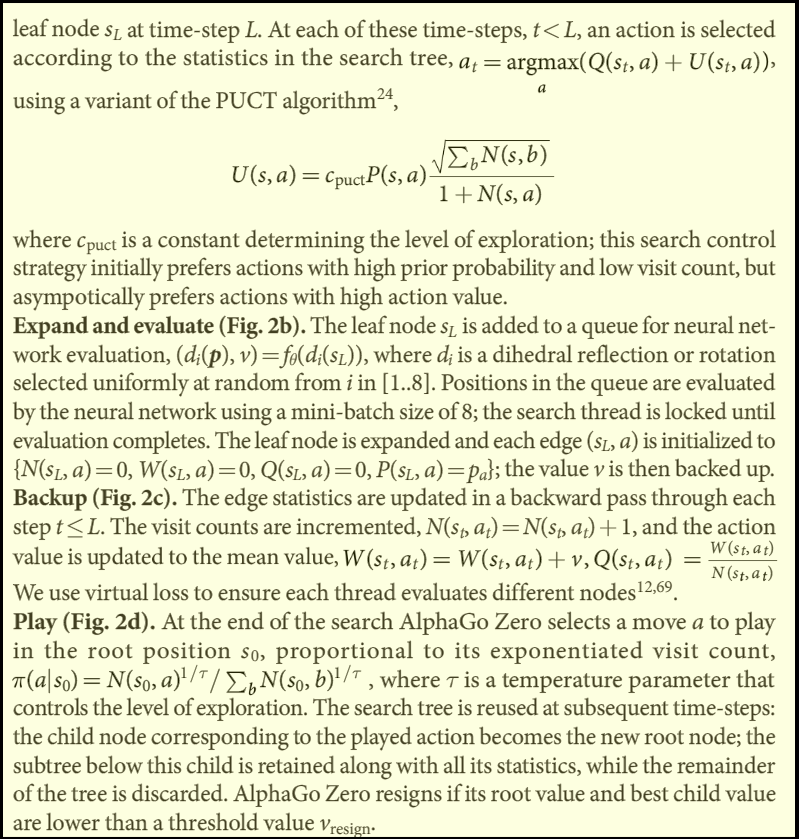
\includegraphics[width=\linewidth, height=1.5in, keepaspectratio]{../figure/alphagozero.png}
\caption{A snippet from the ``methods'' section of the
\href{https://goo.gl/k8pVpL}{``AlphaGo Zero'' paper} by Silver et al,
\emph{Nature}, 2017.}
\label{alphagozerofig}
\end{marginfigure}


\begin{marginfigure}
\centering
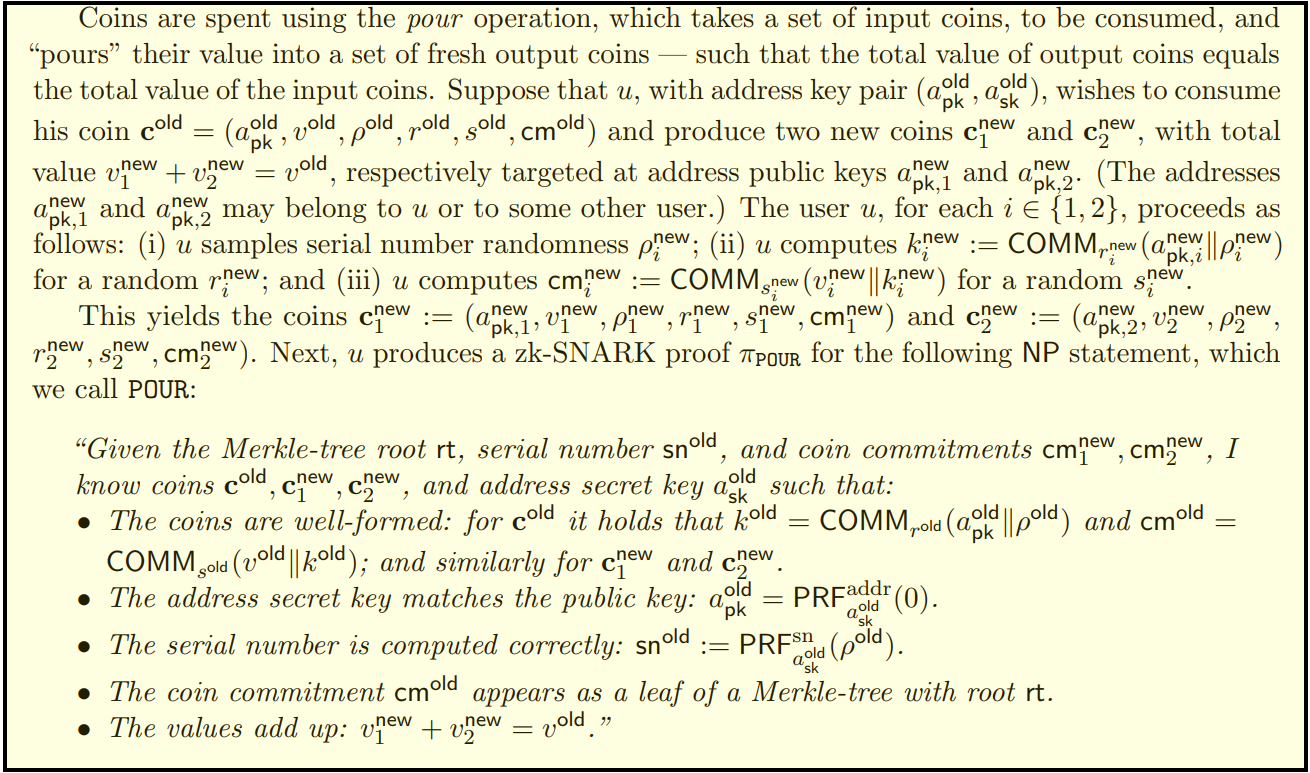
\includegraphics[width=\linewidth, height=1.5in, keepaspectratio]{../figure/zerocash.png}
\caption{A snippet from the
\href{http://zerocash-project.org/paper}{``Zerocash'' paper} of
Ben-Sasson et al, that forms the basis of the cryptocurrency startup
Zcash.}
\label{zerocashfig}
\end{marginfigure}

The basic components of a mathematical text are \textbf{definitions},
\textbf{assertions} and \textbf{proofs}.

\subsection{Definitions}\label{Definitions}

Mathematicians often define new concepts in terms of old concepts.\\
Here is a mathematical definition which you may have encountered in the
past (and will see again shortly):

\hypertarget{onetoonedef}{}
\begin{definition}[One to one function] \label[definition]{onetoonedef}

Let \(S,T\) be sets. We say that a function \(f:S \rightarrow T\) is
\emph{one to one} (also known as \emph{injective}) if for every two
elements \(x,x' \in S\), if \(x \neq x'\) then \(f(x) \neq f(x')\).

\end{definition}

\cref{onetoonedef} captures a simple concept, but even so it uses quite
a bit of notation. When reading such a definition, it is often useful to
annotate it with a pen as you're going through it, as in
\cref{onetoonedefannotatedef}. For example, when you see an identifier
such as \(f\), \(S\) or \(x\), make sure that you realize what sort of
object is it: is it a set, a function, an element, a number, a gremlin?
You might also find it useful to explain the definition in words to a
friend (or to yourself).


\begin{marginfigure}
\centering
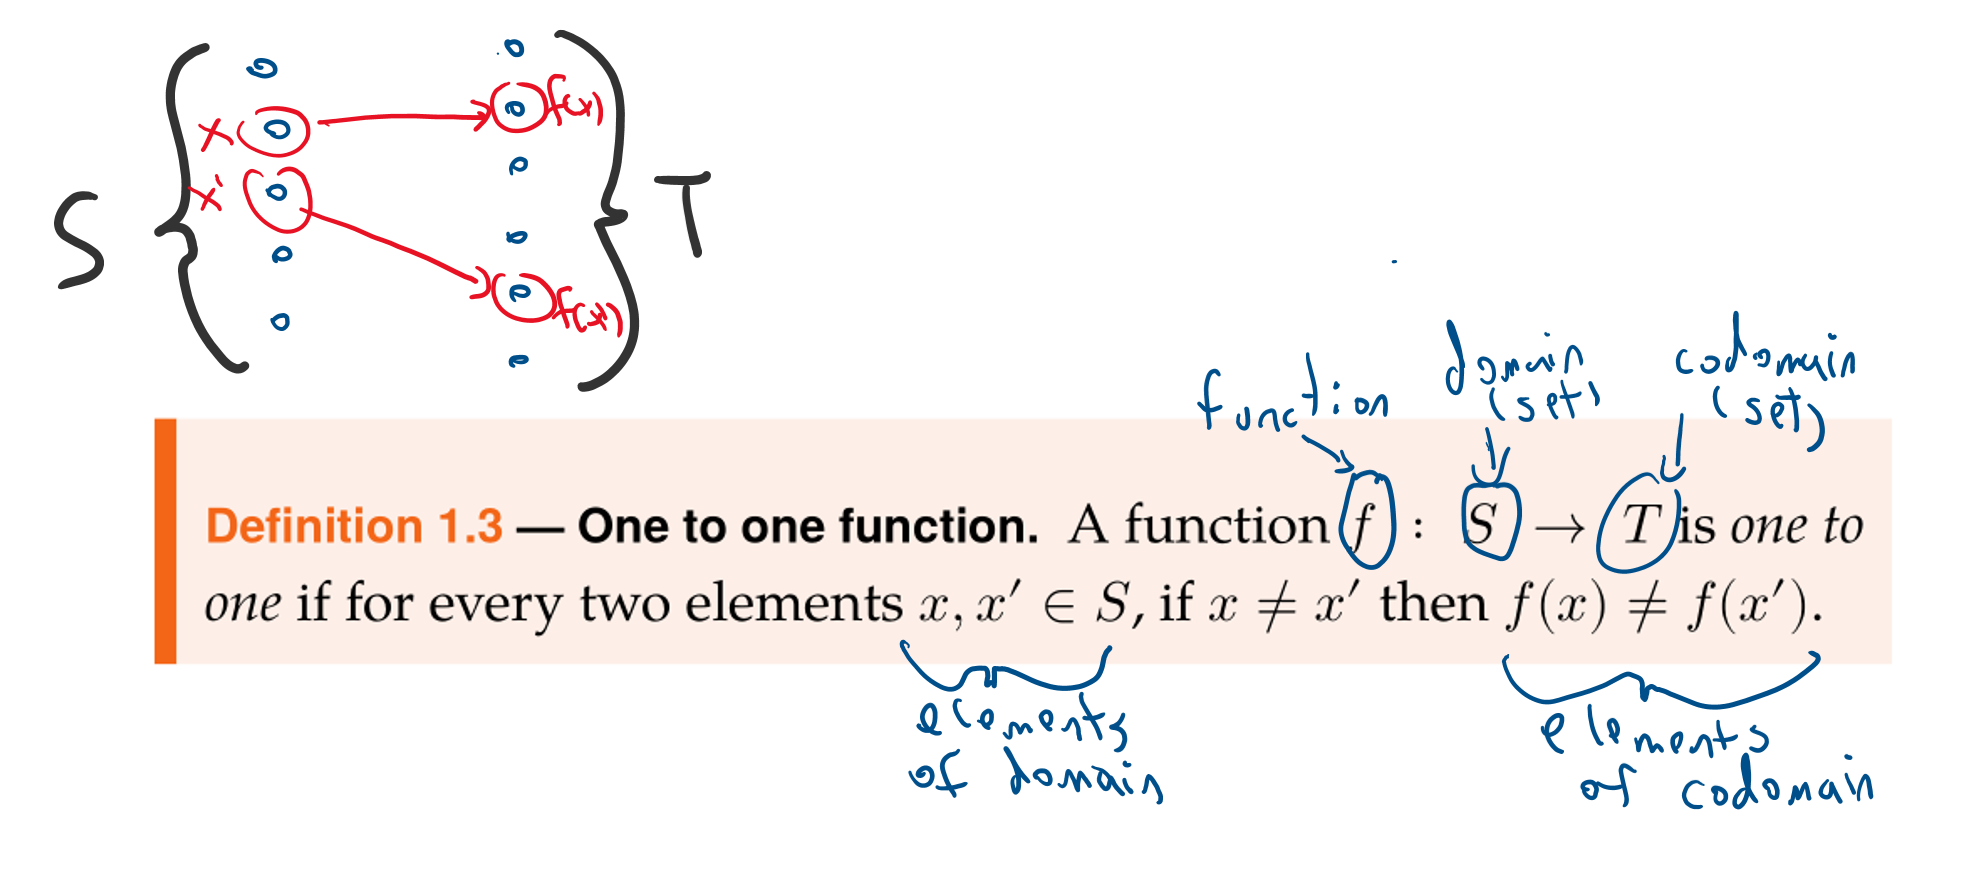
\includegraphics[width=\linewidth, height=1.5in, keepaspectratio]{../figure/onetoonedef.png}
\caption{An annotated form of \cref{onetoonedef}, marking which type is
every object, and with a doodle explaining what the definition says.}
\label{onetoonedefannotatedef}
\end{marginfigure}

\subsection{Assertions: Theorems, lemmas,
claims}\label{Assertions-Theorems-lemma}

Theorems, lemmas, claims and the like are true statements about the
concepts that we defined. Deciding whether to call a particular
statement a ``Theorem'', a ``Lemma'' or a ``Claim'' is a judgement call,
and does not make a mathematical difference. All three correspond to
true statements which can be proven. The difference is that a
\emph{Theorem} refers to a significant result, that we would want to
remember and highlight. A \emph{Lemma} often refers to a technical
result, that is not necessarily important in its own right, but can be
often very useful in proving other theorems. A \emph{Claim} is a ``throw
away'' statement, that we need to use in order to prove some other
bigger results, but do not care so much about for its own sake.

\subsection{Proofs}\label{Proofs}

Mathematical \emph{proofs} are the arguments we use to demonstrate that
our theorems, lemmas, and claims area indeed true. We discuss proofs in
\cref{proofsbackgroundsec} below, but the main point is that the
mathematical standard of proof is very high. Unlike in some other
realms, in mathematics a proof is an ``airtight'' argument that
demonstrates that the statement is true beyond a shadow of a doubt. Some
examples in this section for mathematical proofs are given in
\cref{simplepathlemex} and \cref{topsortsec}. As mentioned in the
preface, as a general rule, it is more important you understand the
\textbf{definitions} than the \textbf{theorems}, and it is more
important you understand a \textbf{theorem statement} than its
\textbf{proof}.

\section{Basic discrete math objects}\label{Basic-discrete-math-objec}

In this section we quickly review some of the mathematical objects (the
``basic data structures'' of mathematics, if you will) we use in this
book.

\subsection{Sets}\label{Sets}

A \emph{set} is an unordered collection of objects. For example, when we
write \(S = \{ 2,4, 7 \}\), we mean that \(S\) denotes the set that
contains the numbers \(2\), \(4\), and \(7\). (We use the notation
``\(2 \in S\)'' to denote that \(2\) is an element of \(S\).) Note that
the set \(\{ 2, 4, 7 \}\) and \(\{ 7 , 4, 2 \}\) are identical, since
they contain the same elements. Also, a set either contains an element
or does not contain it -- there is no notion of containing it ``twice''
-- and so we could even write the same set \(S\) as \(\{ 2, 2, 4, 7\}\)
(though that would be a little weird). The \emph{cardinality} of a
finite set \(S\), denoted by \(|S|\), is the number of elements it
contains. (Cardinality can be defined for \emph{infinite} sets as well;
see the sources in \cref{notesmathchap}.) So, in the example above,
\(|S|=3\). A set \(S\) is a \emph{subset} of a set \(T\), denoted by
\(S \subseteq T\), if every element of \(S\) is also an element of
\(T\). (We can also describe this by saying that \(T\) is a
\emph{superset} of \(S\).) For example,
\(\{2,7\} \subseteq \{ 2,4,7\}\). The set that contains no elements is
known as the \emph{empty set} and it is denoted by \(\emptyset\). If
\(A\) is a subset of \(B\) that is not equal to \(B\) we say that \(A\)
is a \emph{strict subset} of \(B\), and denote this by
\(A \subsetneq B\).

We can define sets by either listing all their elements or by writing
down a rule that they satisfy such as \[
\text{EVEN} = \{ x  \;|\; \text{ $x=2y$ for some non-negative integer $y$} \} \;.
\]

Of course there is more than one way to write the same set, and often we
will use intuitive notation listing a few examples that illustrate the
rule. For example, we can also define \(\text{EVEN}\) as

\[
\text{EVEN} = \{ 0,2,4, \ldots \} \;.
\]

Note that a set can be either finite (such as the set \(\{2,4,7\}\)) or
infinite (such as the set \(\text{EVEN}\)). Also, the elements of a set
don't have to be numbers. We can talk about the sets such as the set
\(\{a,e,i,o,u \}\) of all the vowels in the English language, or the set
\(\{\)\texttt{New York}, \texttt{Los Angeles}, \texttt{Chicago},
\texttt{Houston}, \texttt{Philadelphia}, \texttt{Phoenix},
\texttt{San Antonio}, \texttt{San Diego}, \texttt{Dallas}\(\}\) of all
cities in the U.S. with population more than one million per the 2010
census. A set can even have other sets as elements, such as the set
\(\{ \emptyset, \{1,2\},\{2,3\},\{1,3\} \}\) of all even-sized subsets
of \(\{1,2,3\}\).

\paragraph{Operations on sets:} The \emph{union} of two sets \(S,T\),
denoted by \(S \cup T\), is the set that contains all elements that are
either in \(S\) \emph{or} in \(T\). The \emph{intersection} of \(S\) and
\(T\), denoted by \(S \cap T\), is the set of elements that are both in
\(S\) \emph{and} in \(T\). The \emph{set difference} of \(S\) and \(T\),
denoted by \(S \setminus T\) (and in some texts also by \(S-T\)), is the
set of elements that are in \(S\) but \emph{not} in \(T\).

\paragraph{Tuples, lists, strings, sequences:} A \emph{tuple} is an
\emph{ordered} collection of items. For example \((1,5,2,1)\) is a tuple
with four elements (also known as a \(4\)-tuple or quadruple). Since
order matters, this is not the same tuple as the \(4\)-tuple
\((1,1,5,2)\) or the \(3\)-tuple \((1,5,2)\). A \(2\)-tuple is also
known as a \emph{pair}. We use the terms \emph{tuples} and \emph{lists}
interchangeably. A tuple where every element comes from some finite set
\(\Sigma\) (such as \(\{0,1\}\)) is also known as a \emph{string}.
Analogously to sets, we denote the \emph{length} of a tuple \(T\) by
\(|T|\). Just like sets, we can also think of infinite analogues of
tuples, such as the ordered collection \((1,4,9,\ldots )\) of all
perfect squares. Infinite ordered collections are known as
\emph{sequences}; we might sometimes use the term ``infinite sequence''
to emphasize this, and use ``finite sequence'' as a synonym for a tuple.
(We can identify a sequence \((a_0,a_1,a_2,\ldots)\) of elements in some
set \(S\) with a \emph{function} \(A:\N \rightarrow S\) (where
\(a_n = A(n)\) for every \(n\in \N\)). Similarly, we can identify a
\(k\)-tuple \((a_0,\ldots,a_{k-1})\) of elements in \(S\) with a
function \(A:[k] \rightarrow S\).)

\paragraph{Cartesian product:} If \(S\) and \(T\) are sets, then their
\emph{Cartesian product}, denoted by \(S \times T\), is the set of all
ordered pairs \((s,t)\) where \(s\in S\) and \(t\in T\). For example, if
\(S = \{1,2,3 \}\) and \(T = \{10,12 \}\), then \(S\times T\) contains
the \(6\) elements \((1,10),(2,10),(3,10),(1,12),(2,12),(3,12)\).
Similarly if \(S,T,U\) are sets then \(S\times T \times U\) is the set
of all ordered triples \((s,t,u)\) where \(s\in S\), \(t\in T\), and
\(u\in U\). More generally, for every positive integer \(n\) and sets
\(S_0,\ldots,S_{n-1}\), we denote by
\(S_0 \times S_1 \times \cdots \times S_{n-1}\) the set of ordered
\(n\)-tuples \((s_0,\ldots,s_{n-1})\) where \(s_i\in S_i\) for every
\(i \in \{0,\ldots, n-1\}\). For every set \(S\), we denote the set
\(S\times S\) by \(S^2\), \(S\times S\times S\) by \(S^3\),
\(S\times S\times S \times S\) by \(S^4\), and so on and so forth.

\subsection{Special sets}\label{specialsets}

There are several sets that we will use in this book time and again. The
set

\[
\N = \{ 0, 1,2, \ldots \}
\] contains all \emph{natural numbers}, i.e., non-negative integers. For
any natural number \(n\in\N\), we define the set \([n]\) as
\(\{0,\ldots, n-1\} = \{ k\in \N : k < n \}\). (We start our indexing of
both \(\N\) and \([n]\) from \(0\), while many other texts index those
sets from \(1\). Starting from zero or one is simply a convention that
doesn't make much difference, as long as one is consistent about it.)

We will also occasionally use the set
\(\Z=\{\ldots,-2,-1,0,+1,+2,\ldots \}\) of (negative and non-negative)
\emph{integers},\footnote{The letter Z stands for the German word
  ``Zahlen'', which means \emph{numbers}.} as well as the set \(\R\) of
\emph{real} numbers. (This is the set that includes not just the
integers, but also fractional and irrational numbers; e.g., \(\R\)
contains numbers such as \(+0.5\), \(-\pi\), etc.) We denote by \(\R_+\)
the set \(\{ x\in \R : x > 0 \}\) of \emph{positive} real numbers. This
set is sometimes also denoted as \((0,\infty)\).

\paragraph{Strings:} Another set we will use time and again is

\[
\{0,1\}^n = \{ (x_0,\ldots,x_{n-1}) \;:\; x_0,\ldots,x_{n-1} \in \{0,1\}  \}
\] which is the set of all \(n\)-length binary strings for some natural
number \(n\). That is \(\{0,1\}^n\) is the set of all \(n\)-tuples of
zeroes and ones. This is consistent with our notation above:
\(\{0,1\}^2\) is the Cartesian product \(\{0,1\} \times \{0,1\}\),
\(\{0,1\}^3\) is the product \(\{0,1\} \times \{0,1\} \times \{0,1\}\)
and so on.

We will write the string \((x_0,x_1,\ldots,x_{n-1})\) as simply
\(x_0x_1\cdots x_{n-1}\). For example,

\[
\{0,1\}^3 = \{ 000 , 001, 010 , 011, 100, 101, 110, 111 \} \;.
\]

For every string \(x\in \{0,1\}^n\) and \(i\in [n]\), we write \(x_i\)
for the \(i^{th}\) element of \(x\).

We will also often talk about the set of binary strings of \emph{all}
lengths, which is

\[
\{0,1\}^* = \{ (x_0,\ldots,x_{n-1}) \;:\; n\in\N \;,\;, x_0,\ldots,x_{n-1} \in \{0,1\} \} \;.
\]

Another way to write this set is as \[
\{0,1\}^* = \{0,1\}^0 \cup \{0,1\}^1 \cup \{0,1\}^2 \cup \cdots
\] or more concisely as

\[
\{0,1\}^* = \cup_{n\in\N} \{0,1\}^n \;.
\]

The set \(\{0,1\}^*\) includes the ``string of length \(0\)'' or ``the
empty string'', which we will denote by
\(\ensuremath{\text{\texttt{""}}}\). (In using this notation we follow
the convention of many programming languages. Other texts sometimes use
\(\epsilon\) or \(\lambda\) to denote the empty string.)

\paragraph{Generalizing the star operation:} For every set \(\Sigma\),
we define

\[\Sigma^* = \cup_{n\in \N} \Sigma^n \;.\] For example, if
\(\Sigma = \{a,b,c,d,\ldots,z \}\) then \(\Sigma^*\) denotes the set of
all finite length strings over the alphabet a-z.

\paragraph{Concatenation:} The \emph{concatenation} of two strings
\(x\in \Sigma^n\) and \(y\in \Sigma^m\) is the \((n+m)\)-length string
\(xy\) obtained by writing \(y\) after \(x\). That is, if
\(x \in \{0,1\}^n\) and \(y\in \{0,1\}^m\), then \(xy\) is equal to the
string \(z\in \{0,1\}^{n+m}\) such that for \(i\in [n]\), \(z_i=x_i\)
and for \(i\in \{n,\ldots,n+m-1\}\), \(z_i = y_{i-n}\).

\subsection{Functions}\label{functionsec}

If \(S\) and \(T\) are nonempty sets, a \emph{function} \(F\) mapping
\(S\) to \(T\), denoted by \(F:S \rightarrow T\), associates with every
element \(x\in S\) an element \(F(x)\in T\). The set \(S\) is known as
the \emph{domain} of \(F\) and the set \(T\) is known as the
\emph{codomain} of \(F\). The \emph{image} of a function \(F\) is the
set \(\{ F(x) \;|\; x\in S\}\) which is the subset of \(F\)'s codomain
consisting of all output elements that are mapped from some input. (Some
texts use \emph{range} to denote the image of a function, while other
texts use \emph{range} to denote the codomain of a function. Hence we
will avoid using the term ``range'' altogether.) As in the case of sets,
we can write a function either by listing the table of all the values it
gives for elements in \(S\) or by using a rule. For example if
\(S = \{0,1,2,3,4,5,6,7,8,9 \}\) and \(T = \{0,1 \}\), then the table
below defines a function \(F: S \rightarrow T\). Note that this function
is the same as the function defined by the rule
\(F(x)= (x \mod 2)\).\footnote{For two natural numbers \(x\) and \(a\),
  \(x \mod a\) (shorthand for \href{https://goo.gl/b7Fdzm}{``modulo''})
  denotes the \emph{remainder} of \(x\) when it is divided by \(a\).
  That is, it is the number \(r\) in \(\{0,\ldots,a-1\}\) such that
  \(x = ak +r\) for some integer \(k\). We sometimes also use the
  notation \(x = y\; (\mod a)\) to denote the assertion that
  \(x \mod a\) is the same as \(y \mod a\).}

\begin{longtable}[]{@{}ll@{}}
\caption{An example of a function.}\tabularnewline
\toprule
Input & Output\tabularnewline
\midrule
\endfirsthead
\toprule
Input & Output\tabularnewline
\midrule
\endhead
0 & 0\tabularnewline
1 & 1\tabularnewline
2 & 0\tabularnewline
3 & 1\tabularnewline
4 & 0\tabularnewline
5 & 1\tabularnewline
6 & 0\tabularnewline
7 & 1\tabularnewline
8 & 0\tabularnewline
9 & 1\tabularnewline
\bottomrule
\end{longtable}

If \(f:S \rightarrow T\) satisfies that \(f(x)\neq f(y)\) for all
\(x \neq y\) then we say that \(f\) is \emph{one-to-one}
(\cref{onetoonedef}, also known as an \emph{injective} function or
simply an \emph{injection}). If \(F\) satisfies that for every
\(y\in T\) there is some \(x\in S\) such that \(F(x)=y\) then we say
that \(F\) is \emph{onto} (also known as a \emph{surjective} function or
simply a \emph{surjection}). A function that is both one-to-one and onto
is known as a \emph{bijective} function or simply a \emph{bijection}. A
bijection from a set \(S\) to itself is also known as a
\emph{permutation} of \(S\). If \(F:S \rightarrow T\) is a bijection
then for every \(y\in T\) there is a unique \(x\in S\) such that
\(F(x)=y\). We denote this value \(x\) by \(F^{-1}(y)\). Note that
\(F^{-1}\) is itself a bijection from \(T\) to \(S\) (can you see why?).

Giving a bijection between two sets is often a good way to show they
have the same size. In fact, the standard mathematical definition of the
notion that ``\(S\) and \(T\) have the same cardinality'' is that there
exists a bijection \(f:S \rightarrow T\). Further, the cardinality of a
set \(S\) is defined to be \(n\) if there is a bijection from \(S\) to
the set \(\{0,\ldots,n-1\}\). As we will see later in this book, this is
a definition that generalizes to defining the cardinality of
\emph{infinite} sets.

\paragraph{Partial functions:} We will sometimes be interested in
\emph{partial} functions from \(S\) to \(T\). A partial function is
allowed to be undefined on some subset of \(S\). That is, if \(F\) is a
partial function from \(S\) to \(T\), then for every \(s\in S\), either
there is (as in the case of standard functions) an element \(F(s)\) in
\(T\), or \(F(s)\) is undefined. For example, the partial function
\(F(x)= \sqrt{x}\) is only defined on non-negative real numbers. When we
want to distinguish between partial functions and standard (i.e.,
non-partial) functions, we will call the latter \emph{total} functions.
When we say ``function'' without any qualifier then we mean a
\emph{total} function.

The notion of partial functions is a strict generalization of functions,
and so every function is a partial function, but not every partial
function is a function. (That is, for every nonempty \(S\) and \(T\),
the set of partial functions from \(S\) to \(T\) is a proper superset of
the set of total functions from \(S\) to \(T\).) When we want to
emphasize that a function \(f\) from \(A\) to \(B\) might not be total,
we will write \(f: A \rightarrow_p B\). We can think of a partial
function \(F\) from \(S\) to \(T\) also as a total function from \(S\)
to \(T \cup \{ \bot \}\) where \(\bot\) is a special ``failure symbol''.
So, instead of saying that \(F\) is undefined at \(x\), we can say that
\(F(x)=\bot\).

\paragraph{Basic facts about functions:} Verifying that you can prove
the following results is an excellent way to brush up on functions:

\begin{itemize}
\item
  If \(F:S \rightarrow T\) and \(G:T \rightarrow U\) are one-to-one
  functions, then their \emph{composition} \(H:S \rightarrow U\) defined
  as \(H(s)=G(F(s))\) is also one to one.
\item
  If \(F:S \rightarrow T\) is one to one, then there exists an onto
  function \(G:T \rightarrow S\) such that \(G(F(s))=s\) for every
  \(s\in S\).
\item
  If \(G:T \rightarrow S\) is onto then there exists a one-to-one
  function \(F:S \rightarrow T\) such that \(G(F(s))=s\) for every
  \(s\in S\).
\item
  If \(S\) and \(T\) are finite sets then the following conditions are
  equivalent to one another: \textbf{(a)} \(|S| \leq |T|\), \textbf{(b)}
  there is a one-to-one function \(F:S \rightarrow T\), and \textbf{(c)}
  there is an onto function \(G:T \rightarrow S\). (This is actually
  true even for \emph{infinite} \(S\) and \(T\): in that case
  \textbf{(b)} (or equivalently \textbf{(c)}) is the commonly accepted
  \emph{definition} for \(|S| \leq |T|\).)
\end{itemize}


\begin{marginfigure}
\centering
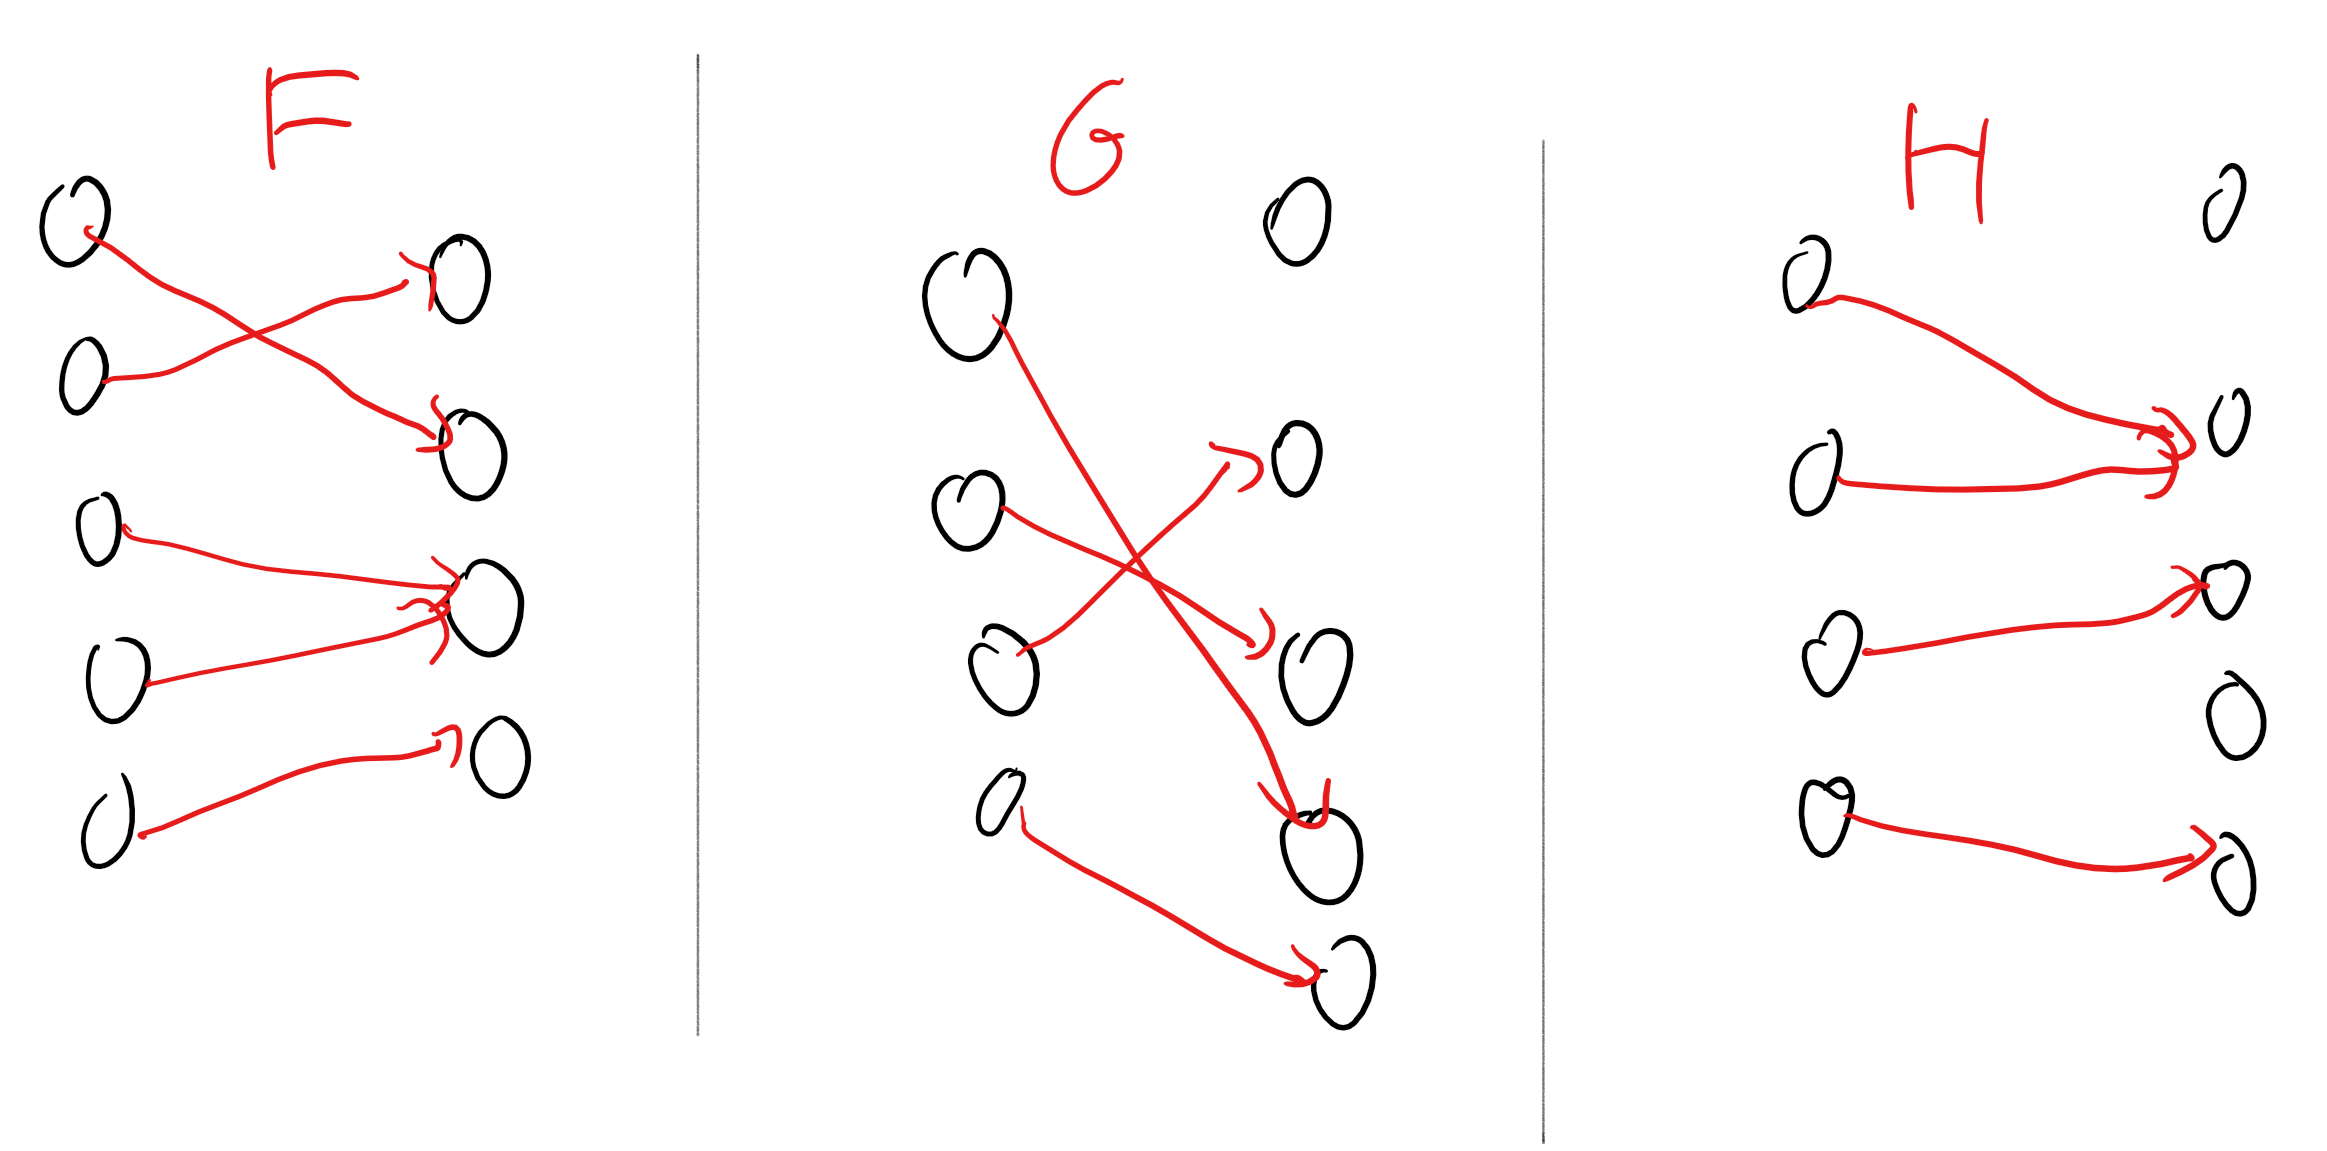
\includegraphics[width=\linewidth, height=1.5in, keepaspectratio]{../figure/functionsdiagram.png}
\caption{We can represent finite functions as a directed graph where we
put an edge from \(x\) to \(f(x)\). The \emph{onto} condition
corresponds to requiring that every vertex in the codomain of the
function has in-degree \emph{at least} one. The \emph{one-to-one}
condition corresponds to requiring that every vertex in the codomain of
the function has in-degree \emph{at most} one. In the examples above
\(F\) is an onto function, \(G\) is one to one, and \(H\) is neither
onto nor one to one.}
\label{functionsdiagrampng}
\end{marginfigure}

\begin{pause} \label[pause]{You-can-find-the-proofs-o}

You can find the proofs of these results in many discrete math texts,
including for example, Section 4.5 in the
\href{https://cs121.boazbarak.org/LLM_data_types.pdf}{Lehman-Leighton-Meyer
notes}. However, I strongly suggest you try to prove them on your own,
or at least convince yourself that they are true by proving special
cases of those for small sizes (e.g., \(|S|=3,|T|=4,|U|=5\)).

\end{pause}

Let us prove one of these facts as an example:

\hypertarget{onetooneimpliesonto}{}
\begin{lemma} \label[lemma]{onetooneimpliesonto}

If \(S,T\) are non-empty sets and \(F:S \rightarrow T\) is one to one,
then there exists an onto function \(G:T \rightarrow S\) such that
\(G(F(s))=s\) for every \(s\in S\).

\end{lemma}

\begin{proof} \label[proof]{Choose-some-s-in-S-We-wil}

Choose some \(s_0 \in S\). We will define the function
\(G:T \rightarrow S\) as follows: for every \(t\in T\), if there is some
\(s\in S\) such that \(F(s)=t\) then set \(G(t)=s\) (the choice of \(s\)
is well defined since by the one-to-one property of \(F\), there cannot
be two distinct \(s,s'\) that both map to \(t\)). Otherwise, set
\(G(t)=s_0\). Now for every \(s\in S\), by the definition of \(G\), if
\(t=F(s)\) then \(G(t)=G(F(s))=s\). Moreover, this also shows that \(G\)
is \emph{onto}, since it means that for every \(s\in S\) there is some
\(t\), namely \(t=F(s)\), such that \(G(t)=s\).

\end{proof}

\subsection{Graphs}\label{graphsec}

\emph{Graphs} are ubiquitous in Computer Science, and many other fields
as well. They are used to model a variety of data types including social
networks, scheduling constraints, road networks, deep neural nets, gene
interactions, correlations between observations, and a great many more.
Formal definitions of several kinds of graphs are given next, but if you
have not seen graphs before in a course, I urge you to read up on them
in one of the sources mentioned in \cref{notesmathchap}.

Graphs come in two basic flavors: \emph{undirected} and
\emph{directed}.\footnote{It is possible, and sometimes useful, to think
  of an undirected graph as the special case of a directed graph that
  has the special property that for every pair \(u,v\) either both the
  edges \((u,v)\) and \((v,u)\) are present or neither of them is.
  However, in many settings there is a significant difference between
  undirected and directed graphs, and so it's typically best to think of
  them as separate categories.}


\begin{marginfigure}[1.5in]
\centering
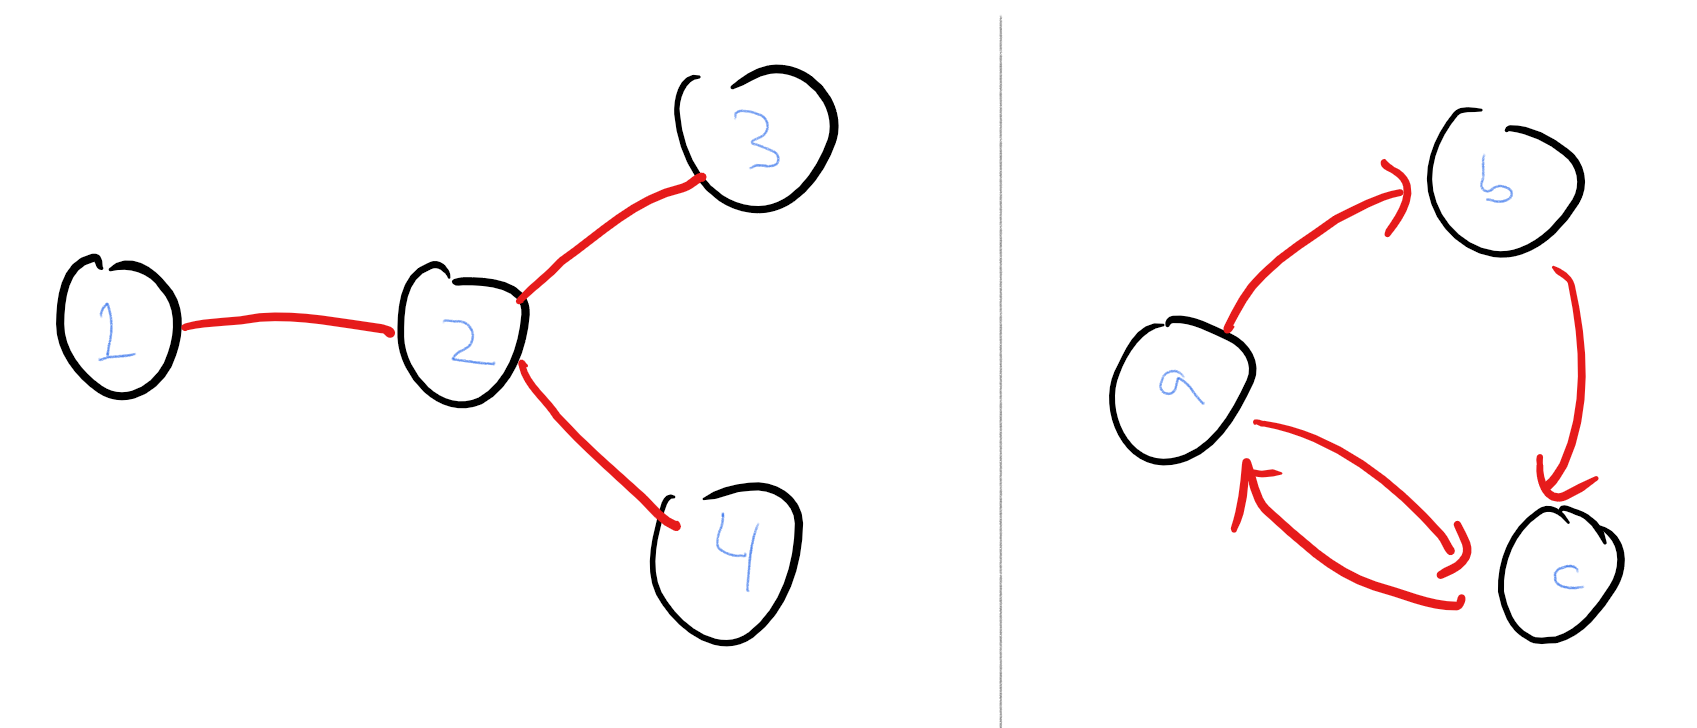
\includegraphics[width=\linewidth, height=1.5in, keepaspectratio]{../figure/graphsexampe.png}
\caption{An example of an undirected and a directed graph. The
undirected graph has vertex set \(\{1,2,3,4\}\) and edge set
\(\{ \{1,2\},\{2,3\},\{2,4\} \}\). The directed graph has vertex set
\(\{a,b,c\}\) and the edge set \(\{ (a,b),(b,c),(c,a),(a,c) \}\).}
\label{graphsexampefig}
\end{marginfigure}

\hypertarget{undirgraph}{}
\begin{definition}[Undirected graphs] \label[definition]{undirgraph}

An \emph{undirected graph} \(G = (V,E)\) consists of a set \(V\) of
\emph{vertices} and a set \(E\) of edges. Every edge is a size two
subset of \(V\). We say that two vertices \(u,v \in V\) are
\emph{neighbors}, if the edge \(\{u,v\}\) is in \(E\).

\end{definition}

Given this definition, we can define several other properties of graphs
and their vertices. We define the \emph{degree} of \(u\) to be the
number of neighbors \(u\) has. A \emph{path} in the graph is a tuple
\((u_0,\ldots,u_k) \in V^{k+1}\), for some \(k>0\) such that \(u_{i+1}\)
is a neighbor of \(u_i\) for every \(i\in [k]\). A \emph{simple path} is
a path \((u_0,\ldots,u_{k-1})\) where all the \(u_i\)'s are distinct. A
\emph{cycle} is a path \((u_0,\ldots,u_k)\) where \(u_0=u_{k}\). We say
that two vertices \(u,v\in V\) are \emph{connected} if either \(u=v\) or
there is a path from \((u_0,\ldots,u_k)\) where \(u_0=u\) and \(u_k=v\).
We say that the graph \(G\) is \emph{connected} if every pair of
vertices in it is connected.

Here are some basic facts about undirected graphs. We give some informal
arguments below, but leave the full proofs as exercises (the proofs can
be found in many of the resources listed in \cref{notesmathchap}).

\hypertarget{degreesegeslem}{}
\begin{lemma} \label[lemma]{degreesegeslem}

In any undirected graph \(G=(V,E)\), the sum of the degrees of all
vertices is equal to twice the number of edges.

\end{lemma}

\cref{degreesegeslem} can be shown by seeing that every edge
\(\{ u,v\}\) contributes twice to the sum of the degrees (once for \(u\)
and the second time for \(v\)).

\hypertarget{conntranslem}{}
\begin{lemma} \label[lemma]{conntranslem}

The connectivity relation is \emph{transitive}, in the sense that if
\(u\) is connected to \(v\), and \(v\) is connected to \(w\), then \(u\)
is connected to \(w\).

\end{lemma}

\cref{conntranslem} can be shown by simply attaching a path of the form
\((u,u_1,u_2,\ldots,u_{k-1},v)\) to a path of the form
\((v,u'_1,\ldots,u'_{k'-1},w)\) to obtain the path
\((u,u_1,\ldots,u_{k-1},v,u'_1,\ldots,u'_{k'-1},w)\) that connects \(u\)
to \(w\).

\hypertarget{simplepathlem}{}
\begin{lemma} \label[lemma]{simplepathlem}

For every undirected graph \(G=(V,E)\) and connected pair \(u,v\), the
shortest path from \(u\) to \(v\) is simple. In particular, for every
connected pair there exists a simple path that connects them.

\end{lemma}

\cref{simplepathlem} can be shown by ``shortcutting'' any non simple
path from \(u\) to \(v\) where the same vertex \(w\) appears twice to
remove it (see \cref{shortcutpathfig}). It is a good exercise to
transforming this intuitive reasoning to a formal proof:


\begin{figure}
\centering
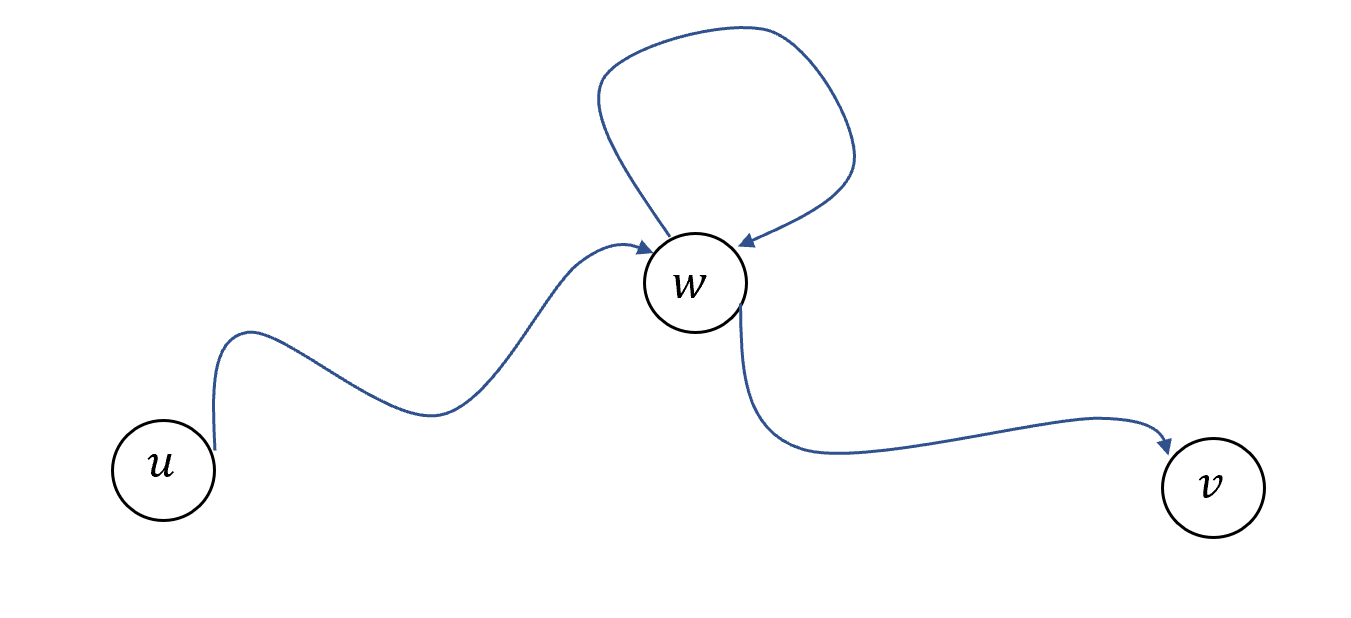
\includegraphics[width=\textwidth, height=0.25\paperheight, keepaspectratio]{../figure/shortcutpath.png}
\caption{If there is a path from \(u\) to \(v\) in a graph that passes
twice through a vertex \(w\) then we can ``shortcut'' it by removing the
loop from \(w\) to itself to find a path from \(u\) to \(v\) that only
passes once through \(w\).}
\label{shortcutpathfig}
\end{figure}

\hypertarget{simplepathlemex}{}
\begin{solvedexercise}[Connected vertices have simple paths] \label[solvedexercise]{simplepathlemex}

Prove \cref{simplepathlem}

\end{solvedexercise}

\begin{solution} \label[solution]{The-proof-follows-the-ide}

The proof follows the idea illustrated in \cref{shortcutpathfig}. One
complication is that there can be more than one vertex that is visited
twice by a path, and so ``shortcutting'' might not necessarily result in
a simple path; we deal with this by looking at a \emph{shortest} path
between \(u\) and \(v\). Details follow.

Let \(G=(V,E)\) be a graph and \(u\) and \(v\) in \(V\) be two connected
vertices in \(G\). We will prove that there is a simple graph between
\(u\) and \(v\). Let \(k\) be the shortest length of a path between
\(u\) and \(v\) and let \(P=(u_0,u_1,u_2,\ldots,u_{k-1},u_k)\) be a
\(k\)-length path from \(u\) to \(v\) (there can be more than one such
path: if so we just choose one of them). (That is \(u_0=u\), \(u_k=v\),
and \((u_\ell,u_{\ell+1})\in E\) for all \(\ell \in [k]\).) We claim
that \(P\) is simple. Indeed, suppose otherwise that there is some
vertex \(w\) that occurs twice in the path: \(w = u_i\) and \(w=u_j\)
for some \(i<j\). Then we can ``shortcut'' the path \(P\) by considering
the path \(P' = (u_0,u_1,\ldots,u_{i-1},w,u_{j+1},\ldots,u_k)\) obtained
by taking the first \(i\) vertices of \(P\) (from \(u_0=0\) to the first
occurrence of \(w\)) and the last \(k-j\) ones (from the vertex
\(u_{j+1}\) following the second occurrence of \(w\) to \(u_k=v\)). The
path \(P'\) is a valid path between \(u\) and \(v\) since every
consecutive pair of vertices in it is connected by an edge (in
particular, since \(w=u_i=w_j\), both \((u_{i-1},w)\) and
\((w,u_{j+1})\) are edges in \(E\)), but since the length of \(P'\) is
\(k-(j-i)<k\), this contradicts the minimality of \(P\).

\end{solution}

\hypertarget{comingupwithproofs}{}
\begin{remark}[Finding proofs] \label[remark]{comingupwithproofs}

\cref{simplepathlemex} is a good example of the process of finding a
proof. You start by ensuring you understand what the statement means,
and then come up with an informal argument why it should be true. You
then transform the informal argument into a rigorous proof. This proof
need not be very long or overly formal, but should clearly establish why
the conclusion of the statement follows from its assumptions.

\end{remark}

The concepts of degrees and connectivity extend naturally to
\emph{directed graphs}, defined as follows.

\hypertarget{directedgraphdef}{}
\begin{definition}[Directed graphs] \label[definition]{directedgraphdef}

A \emph{directed graph} \(G=(V,E)\) consists of a set \(V\) and a set
\(E \subseteq V\times V\) of \emph{ordered pairs} of \(V\). We sometimes
denote the edge \((u,v)\) also as \(u \rightarrow v\). If the edge
\(u \rightarrow v\) is present in the graph then we say that \(v\) is an
\emph{out-neighbor} of \(u\) and \(u\) is an \emph{in-neighbor} of
\(v\).

\end{definition}

A directed graph might contain both \(u \rightarrow v\) and
\(v \rightarrow u\) in which case \(u\) will be both an in-neighbor and
an out-neighbor of \(v\) and vice versa. The \emph{in-degree} of \(u\)
is the number of in-neighbors it has, and the \emph{out-degree} of \(v\)
is the number of out-neighbors it has. A \emph{path} in the graph is a
tuple \((u_0,\ldots,u_k) \in V^{k+1}\), for some \(k>0\) such that
\(u_{i+1}\) is an out-neighbor of \(u_i\) for every \(i\in [k]\). As in
the undirected case, a \emph{simple path} is a path
\((u_0,\ldots,u_{k-1})\) where all the \(u_i\)'s are distinct and a
\emph{cycle} is a path \((u_0,\ldots,u_k)\) where \(u_0=u_{k}\). One
type of directed graphs we often care about is \emph{directed acyclic
graphs} or \emph{DAGs}, which, as their name implies, are directed
graphs without any cycles:

\hypertarget{DAGdef}{}
\begin{definition}[Directed Acyclic Graphs] \label[definition]{DAGdef}

We say that \(G=(V,E)\) is a \emph{directed acyclic graph (DAG)} if it
is a directed graph and there does not exist a list of vertices
\(u_0,u_1,\ldots,u_k \in V\) such that \(u_0=u_k\) and for every
\(i\in [k]\), the edge \(u_i \rightarrow u_{i+1}\) is in \(E\).

\end{definition}

The lemmas we mentioned above have analogs for directed graphs. We again
leave the proofs (which are essentially identical to their undirected
analogs) as exercises.

\hypertarget{diredgreesegeslem}{}
\begin{lemma} \label[lemma]{diredgreesegeslem}

In any directed graph \(G=(V,E)\), the sum of the in-degrees is equal to
the sum of the out-degrees, which is equal to the number of edges.

\end{lemma}

\hypertarget{dirconntranslem}{}
\begin{lemma} \label[lemma]{dirconntranslem}

In any directed graph \(G\), if there is a path from \(u\) to \(v\) and
a path from \(v\) to \(w\), then there is a path from \(u\) to \(w\).

\end{lemma}

\hypertarget{dirsimplepathlem}{}
\begin{lemma} \label[lemma]{dirsimplepathlem}

For every directed graph \(G=(V,E)\) and a pair \(u,v\) such that there
is a path from \(u\) to \(v\), the \emph{shortest path} from \(u\) to
\(v\) is simple.

\end{lemma}

\hypertarget{labeledrem}{}
\begin{remark}[Labeled graphs] \label[remark]{labeledrem}

For some applications we will consider \emph{labeled graphs}, where the
vertices or edges have associated \emph{labels} (which can be numbers,
strings, or members of some other set). We can think of such a graph as
having an associated (possibly partial) \emph{labelling function}
\(L:V \cup E \rightarrow \mathcal{L}\), where \(\mathcal{L}\) is the set
of potential labels. However we will typically not refer explicitly to
this labeling function and simply say things such as ``vertex \(v\) has
the label \(\alpha\)''.

\end{remark}

\subsection{Logic operators and quantifiers}\label{secquantifiers}

If \(P\) and \(Q\) are some statements that can be true or false, then
\(P\) AND \(Q\) (denoted as \(P \wedge Q\)) is a statement that is true
if and only if both \(P\) \emph{and} \(Q\) are true, and \(P\) OR \(Q\)
(denoted as \(P \vee Q\)) is a statement that is true if and only if
either \(P\) \emph{or} \(Q\) is true. The \emph{negation} of \(P\),
denoted as \(\neg P\) or \(\overline{P}\), is true if and only if \(P\)
is false.

Suppose that \(P(x)\) is a statement that depends on some
\emph{parameter} \(x\) (also sometimes known as an \emph{unbound}
variable) in the sense that for every instantiation of \(x\) with a
value from some set \(S\), \(P(x)\) is either true or false. For
example, \(x>7\) is a statement that is not a priori true or false, but
becomes true or false whenever we instantiate \(x\) with some real
number. We denote by \(\forall_{x\in S} P(x)\) the statement that is
true if and only if \(P(x)\) is true \emph{for every}
\(x\in S\).\footnote{In this book, we place the variable bound by a
  quantifier in a subscript and so write \(\forall_{x\in S}P(x)\). Many
  other texts do not use this subscript notation and so will write the
  same statement as \(\forall x\in S, \; P(x)\).} We denote by
\(\exists_{x\in S} P(x)\) the statement that is true if and only if
\emph{there exists} some \(x\in S\) such that \(P(x)\) is true.

For example, the following is a formalization of the true statement that
there exists a natural number \(n\) larger than \(100\) that is not
divisible by \(3\):

\[
\exists_{n\in \N} (n>100) \wedge \left(\forall_{k\in N} k+k+k \neq n\right) \;.
\]

\paragraph{For sufficiently large n.} One expression that we will see
come up time and again in this book is the claim that some statement
\(P(n)\) is true ``for sufficiently large \(n\)''. What this means is
that there exists an integer \(N_0\) such that \(P(n)\) is true for
every \(n>N_0\). We can formalize this as
\(\exists_{N_0\in \N} \forall_{n>N_0} P(n)\).

\subsection{Quantifiers for summations and
products}\label{secquantifierssums}

The following shorthands for summing up or taking products of several
numbers are often convenient. If \(S = \{s_0,\ldots,s_{n-1} \}\) is a
finite set and \(f:S \rightarrow \R\) is a function, then we write
\(\sum_{x\in S} f(x)\) as shorthand for

\[
f(s_0) + f(s_1) + f(s_2) + \ldots + f(s_{n-1}) \;,
\]

and \(\prod_{x\in S} f(x)\) as shorthand for

\[
f(s_0) \cdot f(s_1) \cdot f(s_2) \cdot \ldots \cdot f(s_{n-1}) \;.
\]

For example, the sum of the squares of all numbers from \(1\) to \(100\)
can be written as

\[
\sum_{i\in \{1,\ldots,100\}} i^2 \;. \label{eqsumsquarehundred}
\]

Since summing up over intervals of integers is so common, there is a
special notation for it. For every two integers, \(a \leq b\),
\(\sum_{i=a}^b f(i)\) denotes \(\sum_{i\in S} f(i)\) where
\(S =\{ x\in \Z : a \leq x \leq b \}\). Hence, we can write the sum
\eqref{eqsumsquarehundred} as

\[
\sum_{i=1}^{100} i^2 \;.
\]

\subsection{Parsing formulas: bound and free
variables}\label{boundvarsec}

In mathematics, as in coding, we often have symbolic ``variables'' or
``parameters''. It is important to be able to understand, given some
formula, whether a given variable is \emph{bound} or \emph{free} in this
formula. For example, in the following statement \(n\) is free but \(a\)
and \(b\) are bound by the \(\exists\) quantifier:

\[
\exists_{a,b \in \N} (a \neq 1) \wedge (a \neq n) \wedge (n = a \times b) \label{aboutnstmt}
\]

Since \(n\) is free, it can be set to any value, and the truth of the
statement \eqref{aboutnstmt} depends on the value of \(n\). For example,
if \(n=8\) then \eqref{aboutnstmt} is true, but for \(n=11\) it is
false. (Can you see why?)

The same issue appears when parsing code. For example, in the following
snippet from the C programming language

\begin{code}
for (int i=0 ; i<n ; i=i+1) {
    printf("*");
}
\end{code}

the variable \texttt{i} is bound within the \texttt{for} block but the
variable \texttt{n} is free.

The main property of bound variables is that we can \emph{rename} them
(as long as the new name doesn't conflict with another used variable)
without changing the meaning of the statement. Thus for example the
statement

\[
\exists_{x,y \in \N} (x \neq 1) \wedge (x \neq n) \wedge (n = x \times y) \label{aboutnstmttwo}
\]

is \emph{equivalent} to \eqref{aboutnstmt} in the sense that it is true
for exactly the same set of \(n\)'s.

Similarly, the code

\begin{code}
for (int j=0 ; j<n ; j=j+1) {
    printf("*");
}
\end{code}

produces the same result as the code above that used \texttt{i} instead
of \texttt{j}.

\hypertarget{notationrem}{}
\begin{remark}[Aside: mathematical vs programming notation] \label[remark]{notationrem}

Mathematical notation has a lot of similarities with programming
language, and for the same reasons. Both are formalisms meant to convey
complex concepts in a precise way. However, there are some cultural
differences. In programming languages, we often try to use meaningful
variable names such as \texttt{NumberOfVertices} while in math we often
use short identifiers such as \(n\). Part of it might have to do with
the tradition of mathematical proofs as being handwritten and verbally
presented, as opposed to typed up and compiled. Another reason is if the
wrong variable name is used in a proof, at worst is causes confusion to
readers; when the wrong variable name is used in a program, planes might
crash, patients might die, and rockets could explode.

One consequence of that is that in mathematics we often end up reusing
identifiers, and also ``run out'' of letters and hence use Greek letters
too, as well as distinguish between small and capital letters and
different font faces. Similarly, mathematical notation tends to use
quite a lot of ``overloading'', using operators such as \(+\) for a
great variety of objects (e.g., real numbers, matrices, finite field
elements, etc..), and assuming that the meaning can be inferred from the
context.

Both fields have a notion of ``types'', and in math we often try to
reserve certain letters for variables of a particular type. For example,
variables such as \(i,j,k,\ell,m,n\) will often denote integers, and
\(\epsilon\) will often denote a small positive real number (see
\cref{notationsec} for more on these conventions). When reading or
writing mathematical texts, we usually don't have the advantage of a
``compiler'' that will check type safety for us. Hence it is important
to keep track of the type of each variable, and see that the operations
that are performed on it ``make sense''.

Kun's book \cite{Kun18} contains an extensive discussion on the
similarities and differences between the cultures of mathematics and
programming.

\end{remark}

\subsection{Asymptotics and Big-\(O\) notation}\label{secbigohnotation}

\begin{quote}
\emph{``\(\log\log\log n\) has been proved to go to infinity, but has
never been observed to do so.''}, Anonymous, quoted by Carl Pomerance
(2000)
\end{quote}

It is often very cumbersome to describe precisely quantities such as
running time and is also not needed, since we are typically mostly
interested in the ``higher order terms''. That is, we want to understand
the \emph{scaling behavior} of the quantity as the input variable grows.
For example, as far as running time goes, the difference between an
\(n^5\)-time algorithm and an \(n^2\)-time one is much more significant
than the difference between an \(100n^2 + 10n\) time algorithm and an
\(10n^2\) time algorithm. For this purpose, \(O\)-notation is extremely
useful as a way to ``declutter'' our text and focus our attention on
what really matters. For example, using \(O\)-notation, we can say that
both \(100n^2 + 10n\) and \(10n^2\) are simply \(\Theta(n^2)\) (which
informally means ``the same up to constant factors''), while
\(n^2 = o(n^5)\) (which informally means that \(n^2\) is ``much smaller
than'' \(n^5\)).

Generally (though still informally), if \(F,G\) are two functions
mapping natural numbers to non-negative reals, then ``\(F=O(G)\)'' means
that \(F(n) \leq G(n)\) if we don't care about constant factors, while
``\(F=o(G)\)'' means that \(F\) is much smaller than \(G\), in the sense
that no matter by what constant factor we multiply \(F\), if we take
\(n\) to be large enough then \(G\) will be bigger (for this reason,
sometimes \(F=o(G)\) is written as \(F \ll G\)). We will write
\(F= \Theta(G)\) if \(F=O(G)\) and \(G=O(F)\), which one can think of as
saying that \(F\) is the same as \(G\) if we don't care about constant
factors. More formally, we define Big-\(O\) notation as follows:

\hypertarget{bigohdef}{}
\begin{definition}[Big-$O$ notation] \label[definition]{bigohdef}

Let \(\R_+= \{ x\in \R \;|\; x>0\}\) be the set of positive real
numbers. For two functions \(F,G: \N \rightarrow \R_+\), we say that
\emph{\(F=O(G)\)} if there exist numbers \(a,N_0 \in \N\) such that
\(F(n) \leq a\cdot G(n)\) for every \(n>N_0\). We say that
\(F= \Theta(G)\) if \(F=O(G)\) and \(G=O(F)\). We say that
\(F=\Omega(G)\) if \(G=O(F)\).

We say that \emph{\(F =o(G)\)} if for every \(\epsilon>0\) there is some
\(N_0\) such that \(F(n) <\epsilon G(n)\) for every \(n>N_0\). We say
that \(F =\omega(G)\) if \(G=o(F)\).

\end{definition}


\begin{marginfigure}
\centering
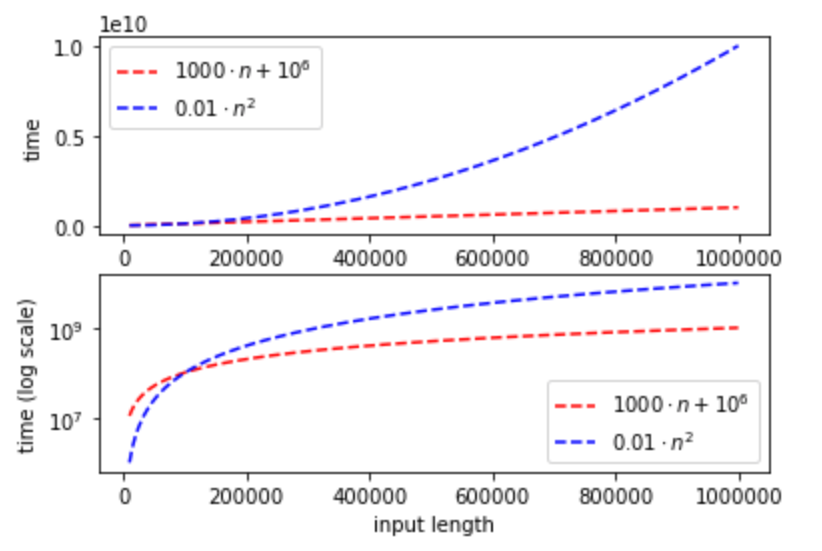
\includegraphics[width=\linewidth, height=1.5in, keepaspectratio]{../figure/nvsnsquared.png}
\caption{If \(F(n)=o(G(n))\) then for sufficiently large \(n\), \(F(n)\)
will be smaller than \(G(n)\). For example, if Algorithm \(A\) runs in
time \(1000\cdot n+10^6\) and Algorithm \(B\) runs in time
\(0.01\cdot n^2\) then even though \(B\) might be more efficient for
smaller inputs, when the inputs get sufficiently large, \(A\) will run
\emph{much} faster than \(B\).}
\label{nvsnsquaredfig}
\end{marginfigure}

It's often convenient to use ``anonymous functions'' in the context of
\(O\)-notation. For example, when we write a statement such as
\(F(n) = O(n^3)\), we mean that \(F=O(G)\) where \(G\) is the function
defined by \(G(n)=n^3\). Chapter 7 in
\href{http://www.cs.yale.edu/homes/aspnes/classes/202/notes.pdf}{Jim
Apsnes' notes on discrete math} provides a good summary of \(O\)
notation; see also \href{http://discrete.gr/complexity/}{this tutorial}
for a gentler and more programmer-oriented introduction.

\emph{\(O\) is not equality.} Using the equality sign for \(O\)-notation
is extremely common, but is somewhat of a misnomer, since a statement
such as \(F = O(G)\) really means that \(F\) is in the set
\(\{ G' : \exists_{N,c} \text{ s.t. } \forall_{n>N} G'(n) \leq c G(n) \}\).
If anything, it makes more sense to use \emph{inequalities} and write
\(F \leq O(G)\) and \(F \geq \Omega(G)\), reserving equality for
\(F = \Theta(G)\), and so we will sometimes use this notation too, but
since the equality notation is quite firmly entrenched we often stick to
it as well. (Some texts write \(F \in O(G)\) instead of \(F = O(G)\),
but we will not use this notation.) Despite the misleading equality
sign, you should remember that a statement such as \(F = O(G)\) means
that \(F\) is ``at most'' \(G\) in some rough sense when we ignore
constants, and a statement such as \(F = \Omega(G)\) means that \(F\) is
``at least'' \(G\) in the same rough sense.

\subsection{Some ``rules of thumb'' for Big-\(O\)
notation}\label{Some-rules-of-thumb-for-B}

There are some simple heuristics that can help when trying to compare
two functions \(F\) and \(G\):

\begin{itemize}
\item
  Multiplicative constants don't matter in \(O\)-notation, and so if
  \(F(n)=O(G(n))\) then \(100F(n)=O(G(n))\).
\item
  When adding two functions, we only care about the larger one. For
  example, for the purpose of \(O\)-notation, \(n^3+100n^2\) is the same
  as \(n^3\), and in general in any polynomial, we only care about the
  larger exponent.
\item
  For every two constants \(a,b>0\), \(n^a = O(n^b)\) if and only if
  \(a \leq b\), and \(n^a = o(n^b)\) if and only if \(a<b\). For
  example, combining the two observations above,
  \(100n^2 + 10n + 100 = o(n^3)\).
\item
  Polynomial is always smaller than exponential:
  \(n^a = o(2^{n^\epsilon})\) for every two constants \(a>0\) and
  \(\epsilon>0\) even if \(\epsilon\) is much smaller than \(a\). For
  example, \(100n^{100} = o(2^{\sqrt{n}})\).
\item
  Similarly, logarithmic is always smaller than polynomial:
  \((\log n)^a\) (which we write as \(\log^a n\)) is \(o(n^\epsilon)\)
  for every two constants \(a,\epsilon>0\). For example, combining the
  observations above, \(100n^2 \log^{100} n = o(n^3)\).
\end{itemize}

\hypertarget{bigonotime}{}
\begin{remark}[Big $O$ for other applications (optional)] \label[remark]{bigonotime}

While Big-\(O\) notation is often used to analyze running time of
algorithms, this is by no means the only application. We can use \(O\)
notation to bound asymptotic relations between any functions mapping
integers to positive numbers. It can be used regardless of whether these
functions are a measure of running time, memory usage, or any other
quantity that may have nothing to do with computation. Here is one
example which is unrelated to this book (and hence one that you can feel
free to skip): one way to state the
\href{https://en.wikipedia.org/wiki/Riemann_hypothesis}{Riemann
Hypothesis} (one of the most famous open questions in mathematics) is
that it corresponds to the conjecture that the number of primes between
\(0\) and \(n\) is equal to \(\int_2^n \tfrac{1}{\ln x} dx\) up to an
additive error of magnitude at most \(O(\sqrt{n}\log n)\).

\end{remark}

\section{Proofs}\label{proofsbackgroundsec}

Many people think of mathematical proofs as a sequence of logical
deductions that starts from some axioms and ultimately arrives at a
conclusion. In fact, some dictionaries
\href{http://www.thefreedictionary.com/mathematical+proof}{define}
proofs that way. This is not entirely wrong, but at its essence
mathematical proof of a statement X is simply an argument that convinces
the reader that X is true beyond a shadow of a doubt.

To produce such a proof you need to:

\begin{enumerate}
\def\labelenumi{\arabic{enumi}.}
\item
  Understand precisely what X means.
\item
  Convince \emph{yourself} that X is true.
\item
  Write your reasoning down in plain, precise and concise English (using
  formulas or notation only when they help clarity).
\end{enumerate}

In many cases, the first part is the most important one. Understanding
what a statement means is oftentimes more than halfway towards
understanding why it is true. In third part, to convince the reader
beyond a shadow of a doubt, we will often want to break down the
reasoning to ``basic steps'', where each basic step is simple enough to
be ``self evident''. The combination of all steps yields the desired
statement.

\subsection{Proofs and programs}\label{Proofs-and-programs}

There is a great deal of similarity between the process of writing
\emph{proofs} and that of writing \emph{programs}, and both require a
similar set of skills. Writing a \emph{program} involves:

\begin{enumerate}
\def\labelenumi{\arabic{enumi}.}
\item
  Understanding what is the \emph{task} we want the program to achieve.
\item
  Convincing \emph{yourself} that the task can be achieved by a
  computer, perhaps by planning on a whiteboard or notepad how you will
  break it up to simpler tasks.
\item
  Converting this plan into code that a compiler or interpreter can
  understand, by breaking up each task into a sequence of the basic
  operations of some programming language.
\end{enumerate}

In programs as in proofs, step 1 is often the most important one. A key
difference is that the reader for proofs is a human being and the reader
for programs is a computer. (This difference is eroding with time as
more proofs are being written in a \emph{machine verifiable} form;
moreover, to ensure correctness and maintainability of programs, it is
important that they can be read and understood by humans.) Thus our
emphasis is on \emph{readability} and having a \emph{clear logical flow}
for our proof (which is not a bad idea for programs as well). When
writing a proof, you should think of your audience as an intelligent but
highly skeptical and somewhat petty reader, that will ``call foul'' at
every step that is not well justified.

\subsection{Proof writing style}\label{Proof-writing-style}

A mathematical proof is a piece of writing, but it is a specific genre
of writing with certain conventions and preferred styles. As in any
writing, practice makes perfect, and it is also important to revise your
drafts for clarity.

In a proof for the statement \(X\), all the text between the words
\textbf{``Proof:''} and \textbf{``QED''} should be focused on
establishing that \(X\) is true. Digressions, examples, or ruminations
should be kept outside these two words, so they do not confuse the
reader. The proof should have a clear logical flow in the sense that
every sentence or equation in it should have some purpose and it should
be crystal-clear to the reader what this purpose is. When you write a
proof, for every equation or sentence you include, ask yourself:

\begin{enumerate}
\def\labelenumi{\arabic{enumi}.}
\item
  Is this sentence or equation stating that some statement is true?
\item
  If so, does this statement follow from the previous steps, or are we
  going to establish it in the next step?
\item
  What is the \emph{role} of this sentence or equation? Is it one step
  towards proving the original statement, or is it a step towards
  proving some intermediate claim that you have stated before?
\item
  Finally, would the answers to questions 1-3 be clear to the reader? If
  not, then you should reorder, rephrase or add explanations.
\end{enumerate}

Some helpful resources on mathematical writing include
\href{https://sites.math.washington.edu/~lee/Writing/writing-proofs.pdf}{this
handout by Lee},
\href{https://math.berkeley.edu/~hutching/teach/proofs.pdf}{this handout
by Hutching}, as well as several of the excellent handouts in
\href{http://web.stanford.edu/class/cs103/}{Stanford's CS 103 class}.

\subsection{Patterns in proofs}\label{Patterns-in-proofs}

\begin{quote}
\emph{``If it was so, it might be; and if it were so, it would be; but
as it isn't, it ain't. That's logic.''}, Lewis Carroll, \emph{Through
the looking-glass}.
\end{quote}

Just like in programming, there are several common patterns of proofs
that occur time and again. Here are some examples:

\paragraph{Proofs by contradiction:} One way to prove that \(X\) is true
is to show that if \(X\) was false it would result in a contradiction.
Such proofs often start with a sentence such as ``Suppose, towards a
contradiction, that \(X\) is false'' and end with deriving some
contradiction (such as a violation of one of the assumptions in the
theorem statement). Here is an example:

\begin{lemma} \label[lemma]{There-are-no-natural-numb}

There are no natural numbers \(a,b\) such that
\(\sqrt{2} = \tfrac{a}{b}\).

\end{lemma}

\begin{proof} \label[proof]{Suppose-towards-a-contrad}

Suppose, towards a contradiction that this is false, and so let
\(a\in \N\) be the smallest number such that there exists some
\(b\in\N\) satisfying \(\sqrt{2}=\tfrac{a}{b}\). Squaring this equation
we get that \(2=a^2/b^2\) or \(a^2=2b^2\) \((*)\). But this means that
\(a^2\) is \emph{even}, and since the product of two odd numbers is odd,
it means that \(a\) is even as well, or in other words, \(a = 2a'\) for
some \(a' \in \N\). Yet plugging this into \((*)\) shows that
\(4a'^2 = 2b^2\) which means \(b^2 = 2a'^2\) is an even number as well.
By the same considerations as above we get that \(b\) is even and hence
\(a/2\) and \(b/2\) are two natural numbers satisfying
\(\tfrac{a/2}{b/2}=\sqrt{2}\), contradicting the minimality of \(a\).

\end{proof}

\paragraph{Proofs of a universal statement:} Often we want to prove a
statement \(X\) of the form ``Every object of type \(O\) has property
\(P\).'' Such proofs often start with a sentence such as ``Let \(o\) be
an object of type \(O\)'' and end by showing that \(o\) has the property
\(P\). Here is a simple example:

\begin{lemma} \label[lemma]{For-every-natural-number-}

For every natural number \(n\in N\), either \(n\) or \(n+1\) is even.

\end{lemma}

\begin{proof} \label[proof]{Let-nin-N-be-some-number-}

Let \(n\in N\) be some number. If \(n/2\) is a whole number then we are
done, since then \(n=2(n/2)\) and hence it is even. Otherwise,
\(n/2+1/2\) is a whole number, and hence \(2(n/2+1/2)=n+1\) is even.

\end{proof}

\paragraph{Proofs of an implication:} Another common case is that the
statement \(X\) has the form ``\(A\) implies \(B\)''. Such proofs often
start with a sentence such as ``Assume that \(A\) is true'' and end with
a derivation of \(B\) from \(A\). Here is a simple example:

\begin{lemma} \label[lemma]{If-b-geq-ac-then-there-is}

If \(b^2 \geq 4ac\) then there is a solution to the quadratic equation
\(ax^2 + bx + c =0\).

\end{lemma}

\begin{proof} \label[proof]{Suppose-that-b-geq-ac-The}

Suppose that \(b^2 \geq 4ac\). Then \(d = b^2 - 4ac\) is a non-negative
number and hence it has a square root \(s\). Thus \(x = (-b+s)/(2a)\)
satisfies \[
\begin{aligned}
ax^2 + bx + c &= a(-b+s)^2/(4a^2) + b(-b+s)/(2a) + c \\
&= (b^2-2bs+s^2)/(4a)+(-b^2+bs)/(2a)+c \;. \label{eq:quadeq}
\end{aligned}
\]

\end{proof}

Rearranging the terms of \eqref{eq:quadeq} we get \[
s^2/(4a)+c- b^2/(4a) = (b^2-4ac)/(4a) + c - b^2/(4a) = 0
\]

\paragraph{Proofs of equivalence:} If a statement has the form ``\(A\)
if and only if \(B\)'' (often shortened as ``\(A\) iff \(B\)'') then we
need to prove both that \(A\) implies \(B\) and that \(B\) implies
\(A\). We call the implication that \(A\) implies \(B\) the ``only if''
direction, and the implication that \(B\) implies \(A\) the ``if''
direction.

\paragraph{Proofs by combining intermediate claims:} When a proof is
more complex, it is often helpful to break it apart into several steps.
That is, to prove the statement \(X\), we might first prove statements
\(X_1\),\(X_2\), and \(X_3\) and then prove that
\(X_1 \wedge X_2 \wedge X_3\) implies \(X\). (Recall that \(\wedge\)
denotes the logical AND operator.)

\paragraph{Proofs by case distinction:} This is a special case of the
above, where to prove a statement \(X\) we split into several cases
\(C_1,\ldots,C_k\), and prove that \textbf{(a)} the cases are
\emph{exhaustive}, in the sense that \emph{one} of the cases \(C_i\)
must happen and \textbf{(b)} go one by one and prove that each one of
the cases \(C_i\) implies the result \(X\) that we are after.

\paragraph{Proofs by induction:} We discuss induction and give an
example in \cref{inductionsec} below. We can think of such proofs as a
variant of the above, where we have an unbounded number of intermediate
claims \(X_0,X_2,\ldots,X_k\), and we prove that \(X_0\) is true, as
well as that \(X_0\) implies \(X_1\), and that \(X_0 \wedge X_1\)
implies \(X_2\), and so on and so forth. The website for CMU course
15-251 contains a
\href{http://www.cs.cmu.edu/~./15251/notes/induction-pitfalls.pdf}{useful
handout} on potential pitfalls when making proofs by induction.

\paragraph{Without loss of generality (w.l.o.g):} This term can be
initially quite confusing. It is essentially a way to simplify proofs by
case distinctions. The idea is that if Case 1 is equal to Case 2 up to a
change of variables or a similar transformation, then the proof of Case
1 will also imply the proof of Case 2. It is always a statement that
should be viewed with suspicion. Whenever you see it in a proof, ask
yourself if you understand \emph{why} the assumption made is truly
without loss of generality, and when you use it, try to see if the use
is indeed justified. When writing a proof, sometimes it might be easiest
to simply repeat the proof of the second case (adding a remark that the
proof is very similar to the first one).

\hypertarget{lamportrem}{}
\begin{remark}[Hierarchical Proofs (optional)] \label[remark]{lamportrem}

Mathematical proofs are ultimately written in English prose. The
well-known computer scientist
\href{https://en.wikipedia.org/wiki/Leslie_Lamport}{Leslie Lamport}
argues that this is a problem, and proofs should be written in a more
formal and rigorous way. In his
\href{https://lamport.azurewebsites.net/pubs/proof.pdf}{manuscript} he
proposes an approach for \emph{structured hierarchical proofs}, that
have the following form:

\begin{itemize}
\item
  A proof for a statement of the form ``If \(A\) then \(B\)'' is a
  sequence of numbered claims, starting with the assumption that \(A\)
  is true, and ending with the claim that \(B\) is true.
\item
  Every claim is followed by a proof showing how it is derived from the
  previous assumptions or claims.
\item
  The proof for each claim is itself a sequence of subclaims.
\end{itemize}

The advantage of Lamport's format is that the role that every sentence
in the proof plays is very clear. It is also much easier to transform
such proofs into machine-checkable forms. The disadvantage is that such
proofs can be tedious to read and write, with less differentiation
between the important parts of the arguments versus the more routine
ones.

\end{remark}

\section{Extended example: Topological Sorting}\label{topsortsec}

In this section we will prove the following: every directed acyclic
graph (DAG, see \cref{DAGdef}) can be arranged in layers so that for all
directed edges \(u \rightarrow v\), the layer of \(v\) is larger than
the layer of \(u\). This result is known as
\href{https://goo.gl/QUskBc}{topological sorting} and is used in many
applications, including task scheduling, build systems, software package
management, spreadsheet cell calculations, and many others (see
\cref{topologicalsortfig}). In fact, we will also use it ourselves later
on in this book.


\begin{figure}
\centering
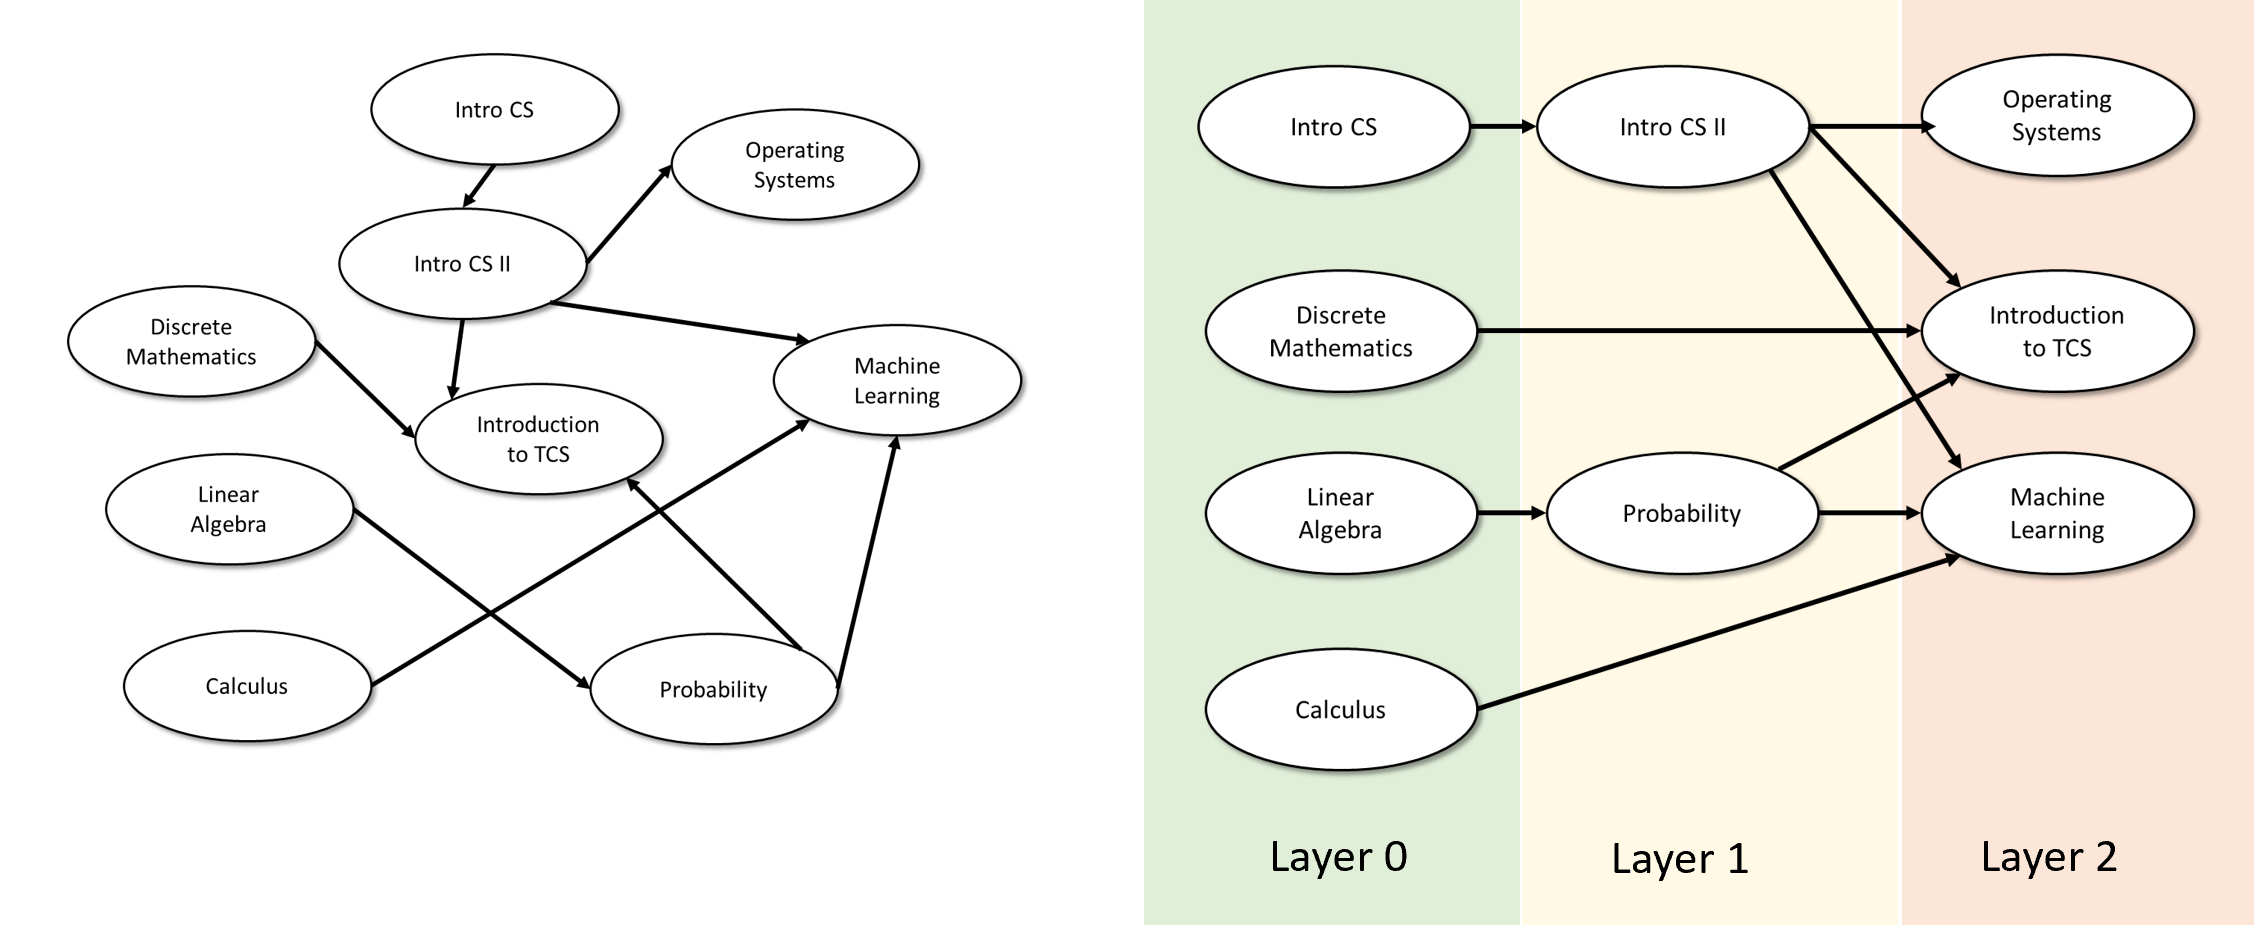
\includegraphics[width=\textwidth, height=0.25\paperheight, keepaspectratio]{../figure/topologicalsort.png}
\caption{An example of \emph{topological sorting}. We consider a
directed graph corresponding to a prerequisite graph of the courses in
some Computer Science program. The edge \(u \rightarrow v\) means that
the course \(u\) is a prerequisite for the course \(v\). A
\emph{layering} or ``topological sorting'' of this graph is the same as
mapping the courses to semesters so that if we decide to take the course
\(v\) in semester \(f(v)\), then we have already taken all the
prerequisites for \(v\) (i.e., its in-neighbors) in prior semesters.}
\label{topologicalsortfig}
\end{figure}

We start with the following definition. A \emph{layering} of a directed
graph is a way to assign for every vertex \(v\) a natural number
(corresponding to its layer), such that \(v\)'s in-neighbors are in
lower-numbered layers than \(v\), and \(v\)'s out-neighbors are in
higher-numbered layers. The formal definition is as follows:

\hypertarget{layeringdef}{}
\begin{definition}[Layering of a DAG] \label[definition]{layeringdef}

Let \(G=(V,E)\) be a directed graph. A \emph{layering} of \(G\) is a
function \(f:V \rightarrow \N\) such that for every edge
\(u \rightarrow v\) of \(G\), \(f(u) < f(v)\).

\end{definition}

In this section we prove that a directed graph is acyclic if and only if
it has a valid layering.

\hypertarget{topologicalsortthm}{}
\begin{theorem}[Topological Sort] \label[theorem]{topologicalsortthm}

Let \(G\) be a directed graph. Then \(G\) is acyclic if and only if
there exists a layering \(f\) of \(G\).

\end{theorem}

To prove such a theorem, we need to first understand what it means.
Since it is an ``if and only if'' statement, \cref{topologicalsortthm}
corresponds to two statements:

\hypertarget{acyclictosortlem}{}
\begin{lemma} \label[lemma]{acyclictosortlem}

For every directed graph \(G\), if \(G\) is acyclic then it has a
layering.

\end{lemma}

\hypertarget{sorttoacycliclem}{}
\begin{lemma} \label[lemma]{sorttoacycliclem}

For every directed graph \(G\), if \(G\) has a layering, then it is
acyclic.

\end{lemma}

To prove \cref{topologicalsortthm} we need to prove both
\cref{acyclictosortlem} and \cref{sorttoacycliclem}.
\cref{sorttoacycliclem} is actually not that hard to prove. Intuitively,
if \(G\) contains a \emph{cycle}, then it cannot be the case that all
edges on the cycle increase in layer number, since if we travel along
the cycle at some point we must come back to the place we started from.
The formal proof is as follows:

\begin{proof} \label[proof]{Let-GVE-be-a-directed-gra}

Let \(G=(V,E)\) be a directed graph and let \(f:V \rightarrow \N\) be a
layering of \(G\) as per \cref{layeringdef} . Suppose, towards a
contradiction, that \(G\) is not acyclic, and hence there exists some
cycle \(u_0,u_1,\ldots,u_k\) such that \(u_0=u_k\) and for every
\(i\in [k]\) the edge \(u_i \rightarrow u_{i+1}\) is present in \(G\).
Since \(f\) is a layering, for every \(i \in [k]\),
\(f(u_i) < f(u_{i+1})\), which means that \[
f(u_0) < f(u_1)  < \cdots  < f(u_k)
\] but this is a contradiction since \(u_0=u_k\) and hence
\(f(u_0)=f(u_k)\).

\end{proof}

\cref{acyclictosortlem} corresponds to the more difficult (and useful)
direction. To prove it, we need to show how given an arbitrary DAG
\(G\), we can come up with a layering of the vertices of \(G\) so that
all edges ``go up''.

\begin{pause} \label[pause]{If-you-have-not-seen-the-}

If you have not seen the proof of this theorem before (or don't remember
it), this would be an excellent point to pause and try to prove it
yourself. One way to do it would be to describe an \emph{algorithm} that
given as input a directed acyclic graph \(G\) on \(n\) vertices and
\(n-2\) or fewer edges, constructs an array \(F\) of length \(n\) such
that for every edge \(u \rightarrow v\) in the graph \(F[u] < F[v]\).

\end{pause}

\subsection{Mathematical induction}\label{inductionsec}

There are several ways to prove \cref{acyclictosortlem}. One approach to
do is to start by proving it for small graphs, such as graphs with 1, 2
or 3 vertices (see \cref{topsortexamplesfig}, for which we can check all
the cases, and then try to extend the proof for larger graphs. The
technical term for this proof approach is \emph{proof by induction}.


\begin{marginfigure}
\centering
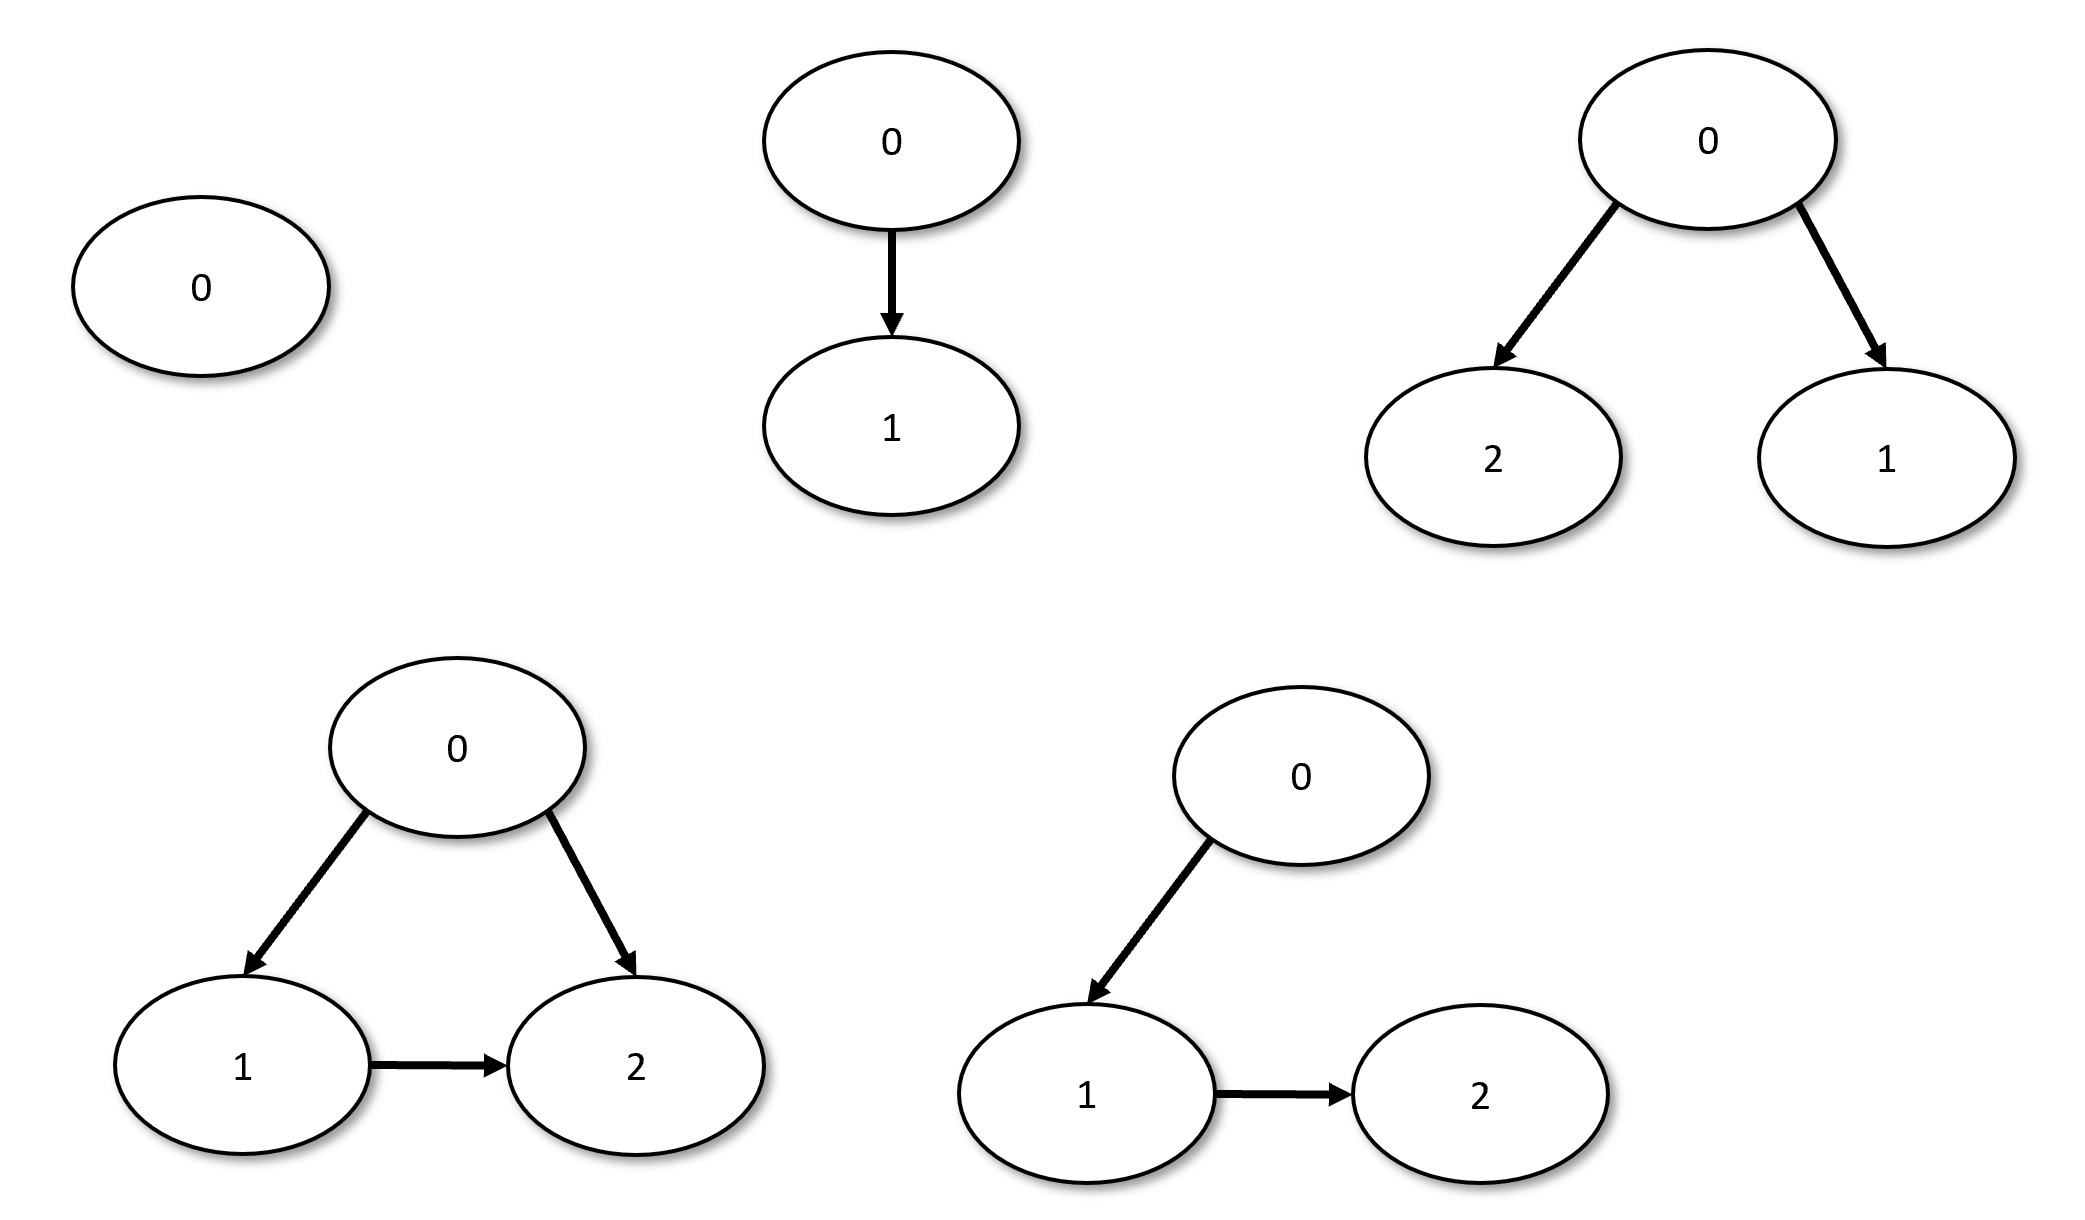
\includegraphics[width=\linewidth, height=1.5in, keepaspectratio]{../figure/topologicalsortexamples.png}
\caption{Some examples of DAGs of one, two and three vertices, and valid
ways to assign layers to the vertices.}
\label{topsortexamplesfig}
\end{marginfigure}

\emph{Induction} is simply an application of the self-evident
\href{https://en.wikipedia.org/wiki/Modus_ponens}{Modus Ponens rule}
that says that if

\paragraph{(a)} \(P\) is true

and

\paragraph{(b)} \(P\) implies \(Q\)

then \(Q\) is true.

In the setting of proofs by induction we typically have a statement
\(Q(k)\) that is parameterized by some integer \(k\), and we prove that
\textbf{(a)} \(Q(0)\) is true, and \textbf{(b)} For every \(k>0\), if
\(Q(0),\ldots,Q(k-1)\) are all true then \(Q(k)\) is true. (Usually
proving \textbf{(b)} is the hard part, though there are examples where
the ``base case'' \textbf{(a)} is quite subtle.) By applying Modus
Ponens, we can deduce from \textbf{(a)} and \textbf{(b)} that \(Q(1)\)
is true. Once we did so, since we now know that both \(Q(0)\) and
\(Q(1)\) are true, then we can use this and \textbf{(b)} to deduce
(again using Modus Ponens) that \(Q(2)\) is true. We can repeat the same
reasoning again and again to obtain that \(Q(k)\) is true for every
\(k\). The statement \textbf{(a)} is called the ``base case'', while
\textbf{(b)} is called the ``inductive step''. The assumption in
\textbf{(b)} that \(Q(i)\) holds for \(i<k\) is called the ``inductive
hypothesis''. (The form of induction described here is sometimes called
``strong induction'' as opposed to ``weak induction'' where we replace
\textbf{(b)} by the statement \textbf{(b')} that if \(Q(k-1)\) is true
then \(Q(k)\) is true; weak induction can be thought of as the special
case of strong induction where we don't use the assumption that
\(Q(0),\ldots,Q(k-2)\) are true.)

\hypertarget{inducrecrem}{}
\begin{remark}[Induction and recursion] \label[remark]{inducrecrem}

Proofs by induction are closely related to algorithms by recursion. In
both cases we reduce solving a larger problem to solving a smaller
instance of itself. In a recursive algorithm to solve some problem P on
an input of length \(k\) we ask ourselves ``what if someone handed me a
way to solve P on instances smaller than \(k\)?''. In an inductive proof
to prove a statement Q parameterized by a number \(k\), we ask ourselves
``what if I already knew that \(Q(k')\) is true for \(k'<k\)?''. Both
induction and recursion are crucial concepts for this course and
Computer Science at large (and even other areas of inquiry, including
not just mathematics but other sciences as well). Both can be confusing
at first, but with time and practice they become clearer. For more on
proofs by induction and recursion, you might find the following
\href{https://cs121.boazbarak.org/StanfordCS103Induction.pdf}{Stanford
CS 103 handout},
\href{https://ocw.mit.edu/courses/electrical-engineering-and-computer-science/6-00sc-introduction-to-computer-science-and-programming-spring-2011/unit-1/lecture-6-recursion/}{this
MIT 6.00 lecture} or
\href{https://cs121.boazbarak.org/LL_induction.pdf}{this excerpt of the
Lehman-Leighton book} useful.

\end{remark}

\subsection{Proving the result by
induction}\label{Proving-the-result-by-ind}

There are several ways to use induction to prove \cref{acyclictosortlem}
by induction. We will use induction on the number \(n\) of vertices, and
so we will define the statement \(Q(n)\) as follows:

\begin{quote}
\(Q(n)\) is \emph{``For every DAG \(G=(V,E)\) with \(n\) vertices, there
is a layering of \(G\).''}
\end{quote}

The statement for \(Q(0)\) (where the graph contains no vertices) is
trivial. Thus it will suffice to prove the following: \emph{for every
\(n>0\), if \(Q(n-1)\) is true then \(Q(n)\) is true.}

To do so, we need to somehow find a way, given a graph \(G\) of \(n\)
vertices, to reduce the task of finding a layering for \(G\) into the
task of finding a layering for some other graph \(G'\) of \(n-1\)
vertices. The idea is that we will find a \emph{source} of \(G\): a
vertex \(v\) that has no in-neighbors. We can then assign to \(v\) the
layer \(0\), and layer the remaining vertices using the inductive
hypothesis in layers \(1,2,\ldots\).

The above is the intuition behind the proof of \cref{acyclictosortlem},
but when writing the formal proof below, we use the benefit of
hindsight, and try to streamline what was a messy journey into a linear
and easy-to-follow flow of logic that starts with the word
\textbf{``Proof:''} and ends with \textbf{``QED''} or the symbol
\(\blacksquare\).\footnote{QED stands for ``quod erat demonstrandum'',
  which is Latin for ``what was to be demonstrated'' or ``the very thing
  it was required to have shown''.} Discussions, examples and
digressions can be very insightful, but we keep them outside the space
delimited between these two words, where (as described by this
\href{http://web.stanford.edu/class/cs103/handouts/120\%20Proofwriting\%20Checklist.pdf}{excellent
handout}) ``every sentence must be load bearing''. Just like we do in
programming, we can break the proof into little ``subroutines'' or
``functions'' (known as \emph{lemmas} or \emph{claims} in math
language), which will be smaller statements that help us prove the main
result. However, the proof should be structured in a way that ensures
that it is always crystal-clear to the reader in what stage we are of
the proof. The reader should be able to tell what is the role of every
sentence in the proof and which part it belongs to. We now present the
formal proof of \cref{acyclictosortlem}.

\begin{proof}[Proof of \cref{acyclictosortlem}] \label[proof]{Let-GVE-be-a-DAG-and-nV-b}

Let \(G=(V,E)\) be a DAG and \(n=|V|\) be the number of its vertices. We
prove the lemma by induction on \(n\). The base case is \(n=0\) where
there are no vertices, and so the statement is trivially true.\footnote{Using
  \(n=0\) as the base case is logically valid, but can be confusing. If
  you find the trivial \(n=0\) case to be confusing, you can always
  directly verify the statement for \(n=1\) and then use both \(n=0\)
  and \(n=1\) as the base cases.} For the case of \(n>0\), we make the
inductive hypothesis that every DAG \(G'\) of at most \(n-1\) vertices
has a layering.

We make the following claim:

\textbf{Claim:} \(G\) must contain a vertex \(v\) of in-degree zero.

\textbf{Proof of Claim:} Suppose otherwise that every vertex \(v\in V\)
has an in-neighbor. Let \(v_0\) be some vertex of \(G\), let \(v_1\) be
an in-neighbor of \(v_0\), \(v_2\) be an in-neighbor of \(v_1\), and
continue in this way for \(n\) steps until we construct a list
\(v_0,v_1,\ldots,v_n\) such that for every \(i\in [n]\), \(v_{i+1}\) is
an in-neighbor of \(v_i\), or in other words the edge
\(v_{i+1} \rightarrow v_i\) is present in the graph. Since there are
only \(n\) vertices in this graph, one of the \(n+1\) vertices in this
sequence must repeat itself, and so there exists \(i<j\) such that
\(v_i=v_j\). But then the sequence
\(v_j \rightarrow v_{j-1} \rightarrow \cdots \rightarrow v_i\) is a
cycle in \(G\), contradicting our assumption that it is acyclic.
\textbf{(QED Claim)}

Given the claim, we can let \(v_0\) be some vertex of in-degree zero in
\(G\), and let \(G'\) be the graph obtained by removing \(v_0\) from
\(G\). \(G'\) has \(n-1\) vertices and hence per the inductive
hypothesis has a layering \(f':(V \setminus \{v_0\}) \rightarrow \N\).
We define \(f:V \rightarrow \N\) as follows:

\[f(v) = \begin{cases}f'(v)+1 & v \neq v_0 \\ 0 & v=v_0 \end{cases}\;.\]

We claim that \(f\) is a valid layering, namely that for every edge
\(u \rightarrow v\), \(f(u) < f(v)\). To prove this, we split into
cases:

\begin{itemize}
\item
  \textbf{Case 1:} \(u \neq v_0\), \(v \neq v_0\). In this case the edge
  \(u \rightarrow v\) exists in the graph \(G'\) and hence by the
  inductive hypothesis \(f'(u) < f'(v)\) which implies that
  \(f'(u)+1 < f'(v)+1\).
\item
  \textbf{Case 2:} \(u=v_0\), \(v \neq v_0\). In this case \(f(u)=0\)
  and \(f(v) = f'(v)+1>0\).
\item
  \textbf{Case 3:} \(u \neq v_0\), \(v=v_0\). This case can't happen
  since \(v_0\) does not have in-neighbors.
\item
  \textbf{Case 4:} \(u=v_0, v=v_0\). This case again can't happen since
  it means that \(v_0\) is its own-neighbor --- it is involved in a
  \emph{self loop} which is a form cycle that is disallowed in an
  acyclic graph.
\end{itemize}

Thus, \(f\) is a valid layering for \(G\) which completes the proof.

\end{proof}

\begin{pause} \label[pause]{Reading-a-proof-is-no-les}

Reading a proof is no less of an important skill than producing one. In
fact, just like understanding code, it is a highly non-trivial skill in
itself. Therefore I strongly suggest that you re-read the above proof,
asking yourself at every sentence whether the assumption it makes is
justified, and whether this sentence truly demonstrates what it purports
to achieve. Another good habit is to ask yourself when reading a proof
for every variable you encounter (such as \(u\), \(i\), \(G'\), \(f'\),
etc. in the above proof) the following questions: \textbf{(1)} What
\emph{type} of variable is it? is it a number? a graph? a vertex? a
function? and \textbf{(2)} What do we know about it? Is it an arbitrary
member of the set? Have we shown some facts about it?, and \textbf{(3)}
What are we \emph{trying} to show about it?.

\end{pause}

\subsection{Minimality and uniqueness}\label{Minimality-and-uniqueness}

\cref{topologicalsortthm} guarantees that for every DAG \(G=(V,E)\)
there exists some layering \(f:V \rightarrow \N\) but this layering is
not necessarily \emph{unique}. For example, if \(f:V \rightarrow \N\) is
a valid layering of the graph then so is the function \(f'\) defined as
\(f'(v) = 2\cdot f(v)\). However, it turns out that the \emph{minimal}
layering is unique. A minimal layering is one where every vertex is
given the smallest layer number possible. We now formally define
minimality and state the uniqueness theorem:

\hypertarget{minimallayeruniquethm}{}
\begin{theorem}[Minimal layering is unique] \label[theorem]{minimallayeruniquethm}

Let \(G=(V,E)\) be a DAG. We say that a layering \(f:V \rightarrow \N\)
is \emph{minimal} if for every vertex \(v \in V\), if \(v\) has no
in-neighbors then \(f(v)=0\) and if \(v\) has in-neighbors then there
exists an in-neighbor \(u\) of \(v\) such that \(f(u) = f(v)-1\).

For every layering \(f,g:V \rightarrow \N\) of \(G\), if both \(f\) and
\(g\) are minimal then \(f=g\).

\end{theorem}

The definition of minimality in \cref{minimallayeruniquethm} implies
that for every vertex \(v \in V\), we cannot move it to a lower layer
without making the layering invalid. If \(v\) is a source (i.e., has
in-degree zero) then a minimal layering \(f\) must put it in layer
\(0\), and for every other \(v\), if \(f(v)=i\), then we cannot modify
this to set \(f(v) \leq i-1\) since there is an-neighbor \(u\) of \(v\)
satisfying \(f(u)=i-1\). What \cref{minimallayeruniquethm} says is that
a minimal layering \(f\) is \emph{unique} in the sense that every other
minimal layering is equal to \(f\).

\begin{proofidea} \label[proofidea]{The-idea-is-to-prove-the-}

The idea is to prove the theorem by induction on the layers. If \(f\)
and \(g\) are minimal then they must agree on the source vertices, since
both \(f\) and \(g\) should assign these vertices to layer \(0\). We can
then show that if \(f\) and \(g\) agree up to layer \(i-1\), then the
minimality property implies that they need to agree in layer \(i\) as
well. In the actual proof we use a small trick to save on writing.
Rather than proving the statement that \(f=g\) (or in other words that
\(f(v)=g(v)\) for every \(v\in V\)), we prove the weaker statement that
\(f(v) \leq g(v)\) for every \(v\in V\). (This is a weaker statement
since the condition that \(f(v)\) is lesser or equal than to \(g(v)\) is
implied by the condition that \(f(v)\) is equal to \(g(v)\).) However,
since \(f\) and \(g\) are just labels we give to two minimal layerings,
by simply changing the names ``\(f\)'' and ``\(g\)'' the same proof also
shows that \(g(v) \leq f(v)\) for every \(v\in V\) and hence that
\(f=g\).

\end{proofidea}

\begin{proof}[Proof of \cref{minimallayeruniquethm}] \label[proof]{Let-GVE-be-a-DAG-and-fgV-}

Let \(G=(V,E)\) be a DAG and \(f,g:V \rightarrow \N\) be two minimal
valid layering of \(G\). We will prove that for every \(v \in V\),
\(f(v) \leq g(v)\). Since we didn't assume anything about \(f,g\) except
their minimality, the same proof will imply that for every \(v\in V\),
\(g(v) \leq f(v)\) and hence that \(f(v)=g(v)\) for every \(v\in V\),
which is what we needed to show.

We will prove that \(f(v) \leq g(v)\) for every \(v \in V\) by induction
on \(i = f(v)\). The case \(i=0\) is immediate: since in this case
\(f(v)=0\), \(g(v)\) must be at least \(f(v)\). For the case \(i>0\), by
the minimality of \(f\), if \(f(v)=i\) then there must exist some
in-neighbor \(u\) of \(v\) such that \(f(u) = i-1\). By the induction
hypothesis we get that \(g(u) \geq i-1\), and since \(g\) is a valid
layering it must hold that \(g(v) > g(u)\) which means that
\(g(v) \geq i = f(v)\).

\end{proof}

\begin{pause} \label[pause]{The-proof-of-crefminimall}

The proof of \cref{minimallayeruniquethm} is fully rigorous, but is
written in a somewhat terse manner. Make sure that you read through it
and understand \emph{why} this is indeed an airtight proof of the
Theorem's statement.

\end{pause}

\section{This book: notation and conventions}\label{notationsec}

Most of the notation we use in this book is standard and is used in most
mathematical texts. The main points where we diverge are:

\begin{itemize}
\item
  We index the natural numbers \(\N\) starting with \(0\) (though many
  other texts, especially in computer science, do the same).
\item
  We also index the set \([n]\) starting with \(0\), and hence define it
  as \(\{0,\ldots,n-1\}\). In other texts it is often defined as
  \(\{1,\ldots, n \}\). Similarly, we index our strings starting with
  \(0\), and hence a string \(x\in \{0,1\}^n\) is written as
  \(x_0x_1\cdots x_{n-1}\).
\item
  If \(n\) is a natural number then \(1^n\) does \emph{not} equal the
  number \(1\) but rather this is the length \(n\) string \(11\cdots 1\)
  (that is a string of \(n\) ones). Similarly, \(0^n\) refers to the
  length \(n\) string \(00 \cdots 0\).
\item
  \emph{Partial} functions are functions that are not necessarily
  defined on all inputs. When we write \(f:A \rightarrow B\) this means
  that \(f\) is a \emph{total} function unless we say otherwise. When we
  want to emphasize that \(f\) can be a partial function, we will
  sometimes write \(f: A \rightarrow_p B\).
\item
  As we will see later on in the course, we will mostly describe our
  computational problems in terms of computing a \emph{Boolean function}
  \(f: \{0,1\}^* \rightarrow \{0,1\}\). In contrast, many other
  textbooks refer to the same task as \emph{deciding a language}
  \(L \subseteq \{0,1\}^*\). These two viewpoints are equivalent, since
  for every set \(L\subseteq \{0,1\}^*\) there is a corresponding
  function \(F\) such that \(F(x)=1\) if and only if \(x\in L\).
  Computing \emph{partial functions} corresponds to the task known in
  the literature as a solving a \emph{promise problem}. Because the
  language notation is so prevalent in other textbooks, we will
  occasionally remind the reader of this correspondence.
\item
  We use \(\ceil{x}\) and \(\floor{x}\) for the ``ceiling'' and
  ``floor'' operators that correspond to ``rounding up'' or ``rounding
  down'' a number to the nearest integer. We use \((x \mod y)\) to
  denote the ``remainder'' of \(x\) when divided by \(y\). That is,
  \((x \mod y) = x - y\floor{x/y}\). In context when an integer is
  expected we'll typically ``silently round'' the quantities to an
  integer. For example, if we say that \(x\) is a string of length
  \(\sqrt{n}\) then this means that \(x\) is of length
  \(\lceil \sqrt{n}\, \rceil\). (We round up for the sake of convention,
  but in most such cases, it will not make a difference whether we round
  up or down.)
\item
  Like most Computer Science texts, we default to the logarithm in base
  two. Thus, \(\log n\) is the same as \(\log_2 n\).
\item
  We will also use the notation \(f(n)=poly(n)\) as a shorthand for
  \(f(n)=n^{O(1)}\) (i.e., as shorthand for saying that there are some
  constants \(a,b\) such that \(f(n) \leq a\cdot n^b\) for every
  sufficiently large \(n\)). Similarly, we will use \(f(n)=polylog(n)\)
  as shorthand for \(f(n)=poly(\log n)\) (i.e., as shorthand for saying
  that there are some constants \(a,b\) such that
  \(f(n) \leq a\cdot (\log n)^b\) for every sufficiently large \(n\)).
\item
  As in often the case in mathematical literature, we use the apostrophe
  character to enrich our set of identifiers. Typically if \(x\) denotes
  some object, then \(x'\), \(x''\), etc. will denote other objects of
  the same type.
\item
  To save on ``cognitive load'' we will often use round constants such
  as \(10,100,1000\) in the statements of both theorems and problem set
  questions. When you see such a ``round'' constant, you can typically
  assume that it has no special significance and was just chosen
  arbitrarily. For example, if you see a theorem of the form ``Algorithm
  \(A\) takes at most \(1000\cdot n^2\) steps to compute function \(F\)
  on inputs of length \(n\)'' then probably the number \(1000\) is an
  abitrary sufficiently large constant, and one could prove the same
  theorem with a bound of the form \(c \cdot n^2\) for a constant \(c\)
  that is smaller than \(1000\). Similarly, if a problem asks you to
  prove that some quantity is at least \(n/100\), it is quite possible
  that in truth the quantity is at least \(n/d\) for some constant \(d\)
  that is smaller than \(100\).
\end{itemize}

\subsection{Variable name conventions}\label{conventionsec}

Like programming, mathematics is full of \emph{variables}. Whenever you
see a variable, it is always important to keep track of what is its
\emph{type} (e.g., whether the variable is a number, a string, a
function, a graph, etc.). To make this easier, we try to stick to
certain conventions and consistently use certain identifiers for
variables of the same type. Some of these conventions are listed in
\cref{notationtable} below. These conventions are not immutable laws and
we might occasionally deviate from them. Also, such conventions do not
replace the need to explicitly declare for each new variable the type of
object that it denotes.

\begin{longtable}[]{@{}ll@{}}
\caption{Conventions for identifiers in this book}\tabularnewline
\toprule
\begin{minipage}[b]{0.11\columnwidth}\raggedright
\emph{Identifier}\strut
\end{minipage} & \begin{minipage}[b]{0.83\columnwidth}\raggedright
\emph{Often denotes object of type}\strut
\end{minipage}\tabularnewline
\midrule
\endfirsthead
\toprule
\begin{minipage}[b]{0.11\columnwidth}\raggedright
\emph{Identifier}\strut
\end{minipage} & \begin{minipage}[b]{0.83\columnwidth}\raggedright
\emph{Often denotes object of type}\strut
\end{minipage}\tabularnewline
\midrule
\endhead
\begin{minipage}[t]{0.11\columnwidth}\raggedright
\(i\),\(j\),\(k\),\(\ell\),\(m\),\(n\)\strut
\end{minipage} & \begin{minipage}[t]{0.83\columnwidth}\raggedright
Natural numbers (i.e., in \(\mathbb{N} = \{0,1,2,\ldots \}\))\strut
\end{minipage}\tabularnewline
\begin{minipage}[t]{0.11\columnwidth}\raggedright
\(\epsilon,\delta\)\strut
\end{minipage} & \begin{minipage}[t]{0.83\columnwidth}\raggedright
Small positive real numbers (very close to \(0\))\strut
\end{minipage}\tabularnewline
\begin{minipage}[t]{0.11\columnwidth}\raggedright
\(x,y,z,w\)\strut
\end{minipage} & \begin{minipage}[t]{0.83\columnwidth}\raggedright
Typically strings in \(\{0,1\}^*\) though sometimes numbers or other
objects. We often identify an object with its representation as a
string.\strut
\end{minipage}\tabularnewline
\begin{minipage}[t]{0.11\columnwidth}\raggedright
\(G\)\strut
\end{minipage} & \begin{minipage}[t]{0.83\columnwidth}\raggedright
A \emph{graph}. The set of \(G\)'s vertices is typically denoted by
\(V\). Often \(V=[n]\). The set of \(G\)'s edges is typically denoted by
\(E\).\strut
\end{minipage}\tabularnewline
\begin{minipage}[t]{0.11\columnwidth}\raggedright
\(S\)\strut
\end{minipage} & \begin{minipage}[t]{0.83\columnwidth}\raggedright
Set\strut
\end{minipage}\tabularnewline
\begin{minipage}[t]{0.11\columnwidth}\raggedright
\(f,g,h\)\strut
\end{minipage} & \begin{minipage}[t]{0.83\columnwidth}\raggedright
Functions. We often (though not always) use lowercase identifiers for
\emph{finite functions}, which map \(\{0,1\}^n\) to \(\{0,1\}^m\) (often
\(m=1\)).\strut
\end{minipage}\tabularnewline
\begin{minipage}[t]{0.11\columnwidth}\raggedright
\(F,G,H\)\strut
\end{minipage} & \begin{minipage}[t]{0.83\columnwidth}\raggedright
Infinite (unbounded input) functions mapping \(\{0,1\}^*\) to
\(\{0,1\}^*\) or \(\{0,1\}^*\) to \(\{0,1\}^m\) for some \(m\). Based on
context, the identifiers \(G,H\) are sometimes used to denote functions
and sometimes graphs.\strut
\end{minipage}\tabularnewline
\begin{minipage}[t]{0.11\columnwidth}\raggedright
\(A,B,C\)\strut
\end{minipage} & \begin{minipage}[t]{0.83\columnwidth}\raggedright
Boolean circuits\strut
\end{minipage}\tabularnewline
\begin{minipage}[t]{0.11\columnwidth}\raggedright
\(M,N\)\strut
\end{minipage} & \begin{minipage}[t]{0.83\columnwidth}\raggedright
Turing machines\strut
\end{minipage}\tabularnewline
\begin{minipage}[t]{0.11\columnwidth}\raggedright
\(P,Q\)\strut
\end{minipage} & \begin{minipage}[t]{0.83\columnwidth}\raggedright
Programs\strut
\end{minipage}\tabularnewline
\begin{minipage}[t]{0.11\columnwidth}\raggedright
\(T\)\strut
\end{minipage} & \begin{minipage}[t]{0.83\columnwidth}\raggedright
A function mapping \(\mathbb{N}\) to \(\mathbb{N}\) that corresponds to
a time bound.\strut
\end{minipage}\tabularnewline
\begin{minipage}[t]{0.11\columnwidth}\raggedright
\(c\)\strut
\end{minipage} & \begin{minipage}[t]{0.83\columnwidth}\raggedright
A positive number (often an unspecified constant; e.g., \(T(n)=O(n)\)
corresponds to the existence of \(c\) s.t. \(T(n) \leq c \cdot n\) every
\(n>0\)). We sometimes use \(a,b\) in a similar way.\strut
\end{minipage}\tabularnewline
\begin{minipage}[t]{0.11\columnwidth}\raggedright
\(\Sigma\)\strut
\end{minipage} & \begin{minipage}[t]{0.83\columnwidth}\raggedright
Finite set (often used as the \emph{alphabet} for a set of
strings).\strut
\end{minipage}\tabularnewline
\bottomrule
\end{longtable}

\label{notationtable}

\subsection{Some idioms}\label{Some-idioms}

Mathematical texts often employ certain conventions or ``idioms''. Some
examples of such idioms that we use in this text include the following:

\begin{itemize}
\item
  \textbf{``Let \(X\) be \(\ldots\)''}, \textbf{``let \(X\) denote
  \(\ldots\)''}, or \textbf{``let \(X= \ldots\)'':} These are all
  different ways for us to say that we are \emph{defining} the symbol
  \(X\) to stand for whatever expression is in the \(\ldots\). When
  \(X\) is a \emph{property} of some objects we might define \(X\) by
  writing something along the lines of \textbf{``We say that \(\ldots\)
  has the property \(X\) if \(\ldots\).''}. While we often try to define
  terms before they are used, sometimes a mathematical sentence reads
  easier if we use a term before defining it, in which case we add
  \textbf{``Where \(X\) is \(\ldots\)''} to explain how \(X\) is defined
  in the preceding expression.
\item
  \textbf{Quantifiers:} Mathematical texts involve many quantifiers such
  as ``for all'' and ``exists''. We sometimes spell these in words as in
  \textbf{``for all \(i\in\N\)''} or \textbf{``there is
  \(x\in \{0,1\}^*\)''}, and sometimes use the formal symbols
  \(\forall\) and \(\exists\). It is important to keep track on which
  variable is quantified in what way the \emph{dependencies} between the
  variables. For example, a sentence fragment such as \textbf{``for
  every \(k >0\) there exists \(n\)''} means that \(n\) can be chosen in
  a way that \emph{depends} on \(k\). The order of quantifiers is
  important. For example, the following is a true statement: \emph{``for
  every natural number \(k>1\) there exists a prime number \(n\) such
  that \(n\) divides \(k\).''} In contrast, the following statement is
  false: \emph{``there exists a prime number \(n\) such that for every
  natural number \(k>1\), \(n\) divides \(k\).''}
\item
  \textbf{Numbered equations, theorems, definitions:} To keep track of
  all the terms we define and statements we prove, we often assign them
  a (typically numeric) label, and then refer back to them in other
  parts of the text.
\item
  \textbf{(i.e.,), (e.g.,):} Mathematical texts tend to contain quite a
  few of these expressions. We use \(X\) (i.e., \(Y\)) in cases where
  \(Y\) is equivalent to \(X\) and \(X\) (e.g., \(Y\)) in cases where
  \(Y\) is an example of \(X\) (e.g., one can use phrases such as ``a
  natural number (i.e., a non-negative integer)'' or ``a natural number
  (e.g., \(7\))'').
\item
  \textbf{``Thus''}, \textbf{``Therefore''} , \textbf{``We get that''}:
  This means that the following sentence is implied by the preceding
  one, as in ``The \(n\)-vertex graph \(G\) is connected. Therefore it
  contains at least \(n-1\) edges.'' We sometimes use
  \textbf{``indeed''} to indicate that the following text justifies the
  claim that was made in the preceding sentence as in \emph{``The
  \(n\)-vertex graph \(G\) has at least \(n-1\) edges. Indeed, this
  follows since \(G\) is connected.''}
\item
  \textbf{Constants:} In Computer Science, we typically care about how
  our algorithms' resource consumption (such as running time)
  \emph{scales} with certain quantities (such as the length of the
  input). We refer to quantities that do not depend on the length of the
  input as \emph{constants} and so often use statements such as
  \emph{``there exists a constant \(c>0\) such that for every
  \(n\in \N\), Algorithm \(A\) runs in at most \(c \cdot n^2\) steps on
  inputs of length \(n\).''} The qualifier ``constant'' for \(c\) is not
  strictly needed but is added to emphasize that \(c\) here is a fixed
  number independent of \(n\). In fact sometimes, to reduce cognitive
  load, we will simply replace \(c\) by a sufficiently large round
  number such as \(10\), \(100\), or \(1000\), or use \(O\)-notation and
  write \emph{``Algorithm \(A\) runs in \(O(n^2)\) time.''}
\end{itemize}

\begin{recap} \label[recap]{The-basic-mathematical-da}

\begin{itemize}
\tightlist
\item
  The basic ``mathematical data structures'' we'll need are
  \emph{numbers}, \emph{sets}, \emph{tuples}, \emph{strings},
  \emph{graphs} and \emph{functions}.
\item
  We can use basic objects to define more complex notions. For example,
  \emph{graphs} can be defined as a list of \emph{pairs}.
\item
  Given precise \emph{definitions} of objects, we can state unambiguous
  and precise \emph{statements}. We can then use mathematical
  \emph{proofs} to determine whether these statements are true or false.
\item
  A mathematical proof is not a formal ritual but rather a clear,
  precise and ``bulletproof'' argument certifying the truth of a certain
  statement.
\item
  Big-\(O\) notation is an extremely useful formalism to suppress less
  significant details and allow us to focus on the high level behavior
  of quantities of interest.
\item
  The only way to get comfortable with mathematical notions is to apply
  them in the contexts of solving problems. You should expect to need to
  go back time and again to the definitions and notation in this chapter
  as you work through problems in this course.
\end{itemize}

\end{recap}

\section{Exercises}\label{Exercises}

\hypertarget{logicalex}{}
\begin{exercise}[Logical expressions] \label[exercise]{logicalex}

\begin{enumerate}
\def\labelenumi{\alph{enumi}.}
\item
  Write a logical expression \(\varphi(x)\) involving the variables
  \(x_0,x_1,x_2\) and the operators \(\wedge\) (AND), \(\vee\) (OR), and
  \(\neg\) (NOT), such that \(\varphi(x)\) is true if the majority of
  the inputs are \emph{True}.
\item
  Write a logical expression \(\varphi(x)\) involving the variables
  \(x_0,x_1,x_2\) and the operators \(\wedge\) (AND), \(\vee\) (OR), and
  \(\neg\) (NOT), such that \(\varphi(x)\) is true if the sum
  \(\sum_{i=0}^{2} x_i\) (identifying ``true'' with \(1\) and ``false''
  with \(0\)) is \emph{odd}.
\end{enumerate}

\end{exercise}

\hypertarget{quantifiersex}{}
\begin{exercise}[Quantifiers] \label[exercise]{quantifiersex}

Use the logical quantifiers \(\forall\) (for all), \(\exists\) (there
exists), as well as \(\wedge,\vee,\neg\) and the arithmetic operations
\(+,\times,=,>,<\) to write the following:

\begin{enumerate}
\def\labelenumi{\alph{enumi}.}
\item
  An expression \(\varphi(n,k)\) such that for every natural numbers
  \(n,k\), \(\varphi(n,k)\) is true if and only if \(k\) divides \(n\).
\item
  An expression \(\varphi(n)\) such that for every natural number \(n\),
  \(\varphi(n)\) is true if and only if \(n\) is a power of three.
\end{enumerate}

\end{exercise}

\begin{exercise} \label[exercise]{Describe-the-following-st}

Describe the following statement in English words:
\(\forall_{n\in\N} \exists_{p>n} \forall{a,b \in \N} (a\times b \neq p) \vee (a=1)\).

\end{exercise}

\hypertarget{setsdescription}{}
\begin{exercise}[Set construction notation] \label[exercise]{setsdescription}

Describe in words the following sets:

\begin{enumerate}
\def\labelenumi{\alph{enumi}.}
\item
  \(S = \{ x\in \{0,1\}^{100} : \forall_{i\in \{0,\ldots, 99\}} x_i = x_{99-i} \}\)
\item
  \(T = \{ x\in \{0,1\}^* : \forall_{i,j \in \{2,\ldots,|x|-1 \} } i\cdot j \neq |x| \}\)
\end{enumerate}

\end{exercise}

\hypertarget{cardinalitiesex}{}
\begin{exercise}[Existence of one to one mappings] \label[exercise]{cardinalitiesex}

For each one of the following pairs of sets \((S,T)\), prove or disprove
the following statement: there is a one to one function \(f\) mapping
\(S\) to \(T\).

\begin{enumerate}
\def\labelenumi{\alph{enumi}.}
\item
  Let \(n>10\). \(S = \{0,1\}^n\) and \(T= [n] \times [n] \times [n]\).
\item
  Let \(n>10\). \(S\) is the set of all functions mapping \(\{0,1\}^n\)
  to \(\{0,1\}\). \(T = \{0,1\}^{n^3}\).
\item
  Let \(n>100\). \(S = \{k \in [n] \;|\; k \text{ is prime} \}\),
  \(T = \{0,1\}^{\ceil{\log n -1}}\).
\end{enumerate}

\end{exercise}

\hypertarget{inclex}{}
\begin{exercise}[Inclusion Exclusion] \label[exercise]{inclex}

\begin{enumerate}
\def\labelenumi{\alph{enumi}.}
\item
  Let \(A,B\) be finite sets. Prove that
  \(|A\cup B| = |A|+|B|-|A\cap B|\).
\item
  Let \(A_0,\ldots,A_{k-1}\) be finite sets. Prove that
  \(|A_0 \cup \cdots \cup A_{k-1}| \geq \sum_{i=0}^{k-1} |A_i| - \sum_{0 \leq i < j < k} |A_i \cap A_j|\).
\item
  Let \(A_0,\ldots,A_{k-1}\) be finite subsets of \(\{1,\ldots, n\}\),
  such that \(|A_i|=m\) for every \(i\in [k]\). Prove that if
  \(k>100n\), then there exist two distinct sets \(A_i,A_j\) s.t.
  \(|A_i \cap A_j| \geq m^2/(10n)\).
\end{enumerate}

\end{exercise}

\begin{exercise} \label[exercise]{Prove-that-if-ST-are-fini}

Prove that if \(S,T\) are finite and \(F:S \rightarrow T\) is one to one
then \(|S| \leq |T|\).

\end{exercise}

\begin{exercise} \label[exercise]{Prove-that-if-ST-are-fini}

Prove that if \(S,T\) are finite and \(F:S \rightarrow T\) is onto then
\(|S| \geq |T|\).

\end{exercise}

\begin{exercise} \label[exercise]{Prove-that-for-every-fini}

Prove that for every finite \(S,T\), there are \((|T|+1)^{|S|}\) partial
functions from \(S\) to \(T\).

\end{exercise}

\begin{exercise} \label[exercise]{Suppose-that--Sn-nin-N-is}

Suppose that \(\{ S_n \}_{n\in \N}\) is a sequence such that
\(S_0 \leq 10\) and for \(n>1\)
\(S_n \leq 5 S_{\lfloor \tfrac{n}{5} \rfloor} + 2n\). Prove by induction
that \(S_n \leq 100 n \log n\) for every \(n\).

\end{exercise}

\begin{exercise} \label[exercise]{Prove-that-for-every-undi}

Prove that for every undirected graph \(G\) of \(100\) vertices, if
every vertex has degree at most \(4\), then there exists a subset \(S\)
of at \(20\) vertices such that no two vertices in \(S\) are neighbors
of one another.

\end{exercise}

\hypertarget{ohnotationex}{}
\begin{exercise}[$O$-notation] \label[exercise]{ohnotationex}

For every pair of functions \(F,G\) below, determine which of the
following relations holds: \(F=O(G)\), \(F=\Omega(G)\), \(F=o(G)\) or
\(F=\omega(G)\).

\begin{enumerate}
\def\labelenumi{\alph{enumi}.}
\item
  \(F(n)=n\), \(G(n)=100n\).
\item
  \(F(n)=n\), \(G(n)=\sqrt{n}\).
\item
  \(F(n)=n\log n\), \(G(n)=2^{(\log (n))^2}\).
\item
  \(F(n)=\sqrt{n}\), \(G(n)=2^{\sqrt{\log n}}\)
\item
  \(F(n) = \binom{n}{\ceil{0.2 n}}\) , \(G(n) = 2^{0.1 n}\) (where
  \(\binom{n}{k}\) is the number of \(k\)-sized subsets of a set of size
  \(n\)) and \(g(n) = 2^{0.1 n}\). See footnote for hint.\footnote{one
    way to do this is to use \href{https://goo.gl/cqEmS2}{Stirling's
    approximation for the factorial function.}.}
\end{enumerate}

\end{exercise}

\begin{exercise} \label[exercise]{Give-an-example-of-a-pair}

Give an example of a pair of functions \(F,G:\N \rightarrow \N\) such
that neither \(F=O(G)\) nor \(G=O(F)\) holds.

\end{exercise}

\hypertarget{graphcycleex}{}
\begin{exercise} \label[exercise]{graphcycleex}

Prove that for every undirected graph \(G\) on \(n\) vertices, if \(G\)
has at least \(n\) edges then \(G\) contains a cycle.

\end{exercise}

\hypertarget{indsetex}{}
\begin{exercise} \label[exercise]{indsetex}

Prove that for every undirected graph \(G\) of \(1000\) vertices, if
every vertex has degree at most \(4\), then there exists a subset \(S\)
of at least \(200\) vertices such that no two vertices in \(S\) are
neighbors of one another.

\end{exercise}

\section{Bibliographical notes}\label{notesmathchap}

The heading ``A Mathematician's Apology'', refers to Hardy's classic
book \cite{Hardy41}. Even when Hardy is wrong, he is very much worth
reading.

There are many online sources for the mathematical background needed for
this book. In particular, the lecture notes for MIT 6.042 ``Mathematics
for Computer Science'' \cite{LehmanLeightonMeyer} are extremely
comprehensive, and videos and assignments for this course are available
online. Similarly, \href{http://www.eecs70.org/}{Berkeley CS 70:
``Discrete Mathematics and Probability Theory''} has extensive lecture
notes online.

Other sources for discrete mathematics are Rosen \cite{Rosen19discrete}
and Jim Aspens' online book \cite{AspensDiscreteMath}. Lewis and Zax
\cite{LewisZax19}, as well as the online book of Fleck \cite{Fleck},
give a more gentle overview of the much of the same material. Solow
\cite{Solow14} is a good introduction to proof reading and writing. Kun
\cite{Kun18} gives an introduction to mathematics aimed at readers with
programming background. Stanford's \href{https://cs103.stanford.edu}{CS
103 course} has a wonderful collections of handouts on mathematical
proof techniques and discrete mathematics.

The word \emph{graph} in the sense of \cref{undirgraph} was coined by
the mathematician Sylvester in 1878 in analogy with the chemical graphs
used to visualize molecules. There is an unfortunate confusion between
this term and the more common usage of the word ``graph'' as a way to
plot data, and in particular a plot of some function \(f(x)\) as a
function of \(x\). One way to relate these two notions is to identify
every function \(f:A \rightarrow B\) with the directed graph \(G_f\)
over the vertex set \(V= A \cup B\) such that \(G_f\) contains the edge
\(x \rightarrow f(x)\) for every \(x\in A\). In a graph \(G_f\)
constructed in this way, every vertex in \(A\) has out-degree equal to
one. If the function \(f\) is \emph{one to one} then every vertex in
\(B\) has in-degree at most one. If the function \(f\) is \emph{onto}
then every vertex in \(B\) has in-degree at least one. If \(f\) is a
bijection then every vertex in \(B\) has in-degree exactly equal to one.

Carl Pomerance's quote is taken from
\href{http://sites.math.rutgers.edu/~zeilberg/quotes.html}{the home page
of Doron Zeilberger}.
